\chapter{Learning neither General, nor Specific, but Significant Representations}
\label{chap:2}

\section{Introduction}
Humans instinctively know how to efficiently ``select details'' that are useful for recognition and at the same time ``abstract away'' unnecessary or noisy details.~\cite{tenenbaum2011grow, gentner1997structure, battaglia2018relational} 
This is, in fact, a survival trait, since we cannot possibly save all the detail around us in our brain. Hence, to define objects and actions, we can extract a subset from an extensive but finite set of existing features that are neither \emph{too specific}, nor \emph{too general}, but \emph{significant}. In many cases, this is done by analyzing inheritance (is-a) and composition (has-a) relationships between concepts, entities, and actions~\citep{goodwin2005reasoning, botvinick2008hierarchical}. 
Inspired by that, in this chapter, we explore ideas to address one of our research questions:
\resq{c2}


We presents our ideas and discussions in the context of language understanding tasks, in particular modeling textual entities for information retrieval applications. As the modeling approach, we estimate unigram language model, or so-called  ``bag of words'' model, to represent an entity, like a person, organization, category, etc, given a set of texts connected to the entity.  In fact, we assume that the textual documents associated with an entity are samples drawn from the distribution of a model that represents the entity, and then estimate the model given these samples.

More specifically, we introduce \textsl{\swlms}\ (\acswlm)~\cite{Dehghani:CIKM2016:long, Dehghani:2016:CHIIR, Dehghani2016:trec} as a family of models aim at learning representations for an entity, given a set of documents associated with the entity, so that \emph{all, and only}, the significant shared terms are captured in the models. This makes these models to be not only distinctive but also supported by all the documents in the set. In short, this is achieved by adjusting the weights of terms already well explained by the all the existing documents in the collection as well as the weight of terms that are only explained by a specific document in the set, which eventually results in having the significant terms left in the model. 

\definecolor{sp}{HTML}{e92085}
\definecolor{ge}{HTML}{20b7e9}
\definecolor{re}{HTML}{b7e920}
    
\newcommand\gauss[2]{1/(#2*sqrt(20*pi))*exp(-((x-#1)^2)/(0.03*#2^0.5))} % Gauss function, parameters mu and sigma

\begin{figure}[t!]
    \centering
    \begin{tikzpicture}
    \begin{axis}[every axis plot post/.append style={
      mark=none,samples=50,smooth}, % All plots: from -2:2, 50 samples, smooth, no marks
      %grid=both,
    % xlabel style = {font=\fontsize{9}{10}\selectfont},
    % ylabel style = {font=\fontsize{9}{10}\selectfont},
    ylabel=Frequency,
    xlabel=Terms,
    xmax=0.8,
    ymax=0.5,
    width=11cm,%\textwidth,
    height=6cm, %5cm,
    xtick=\empty, 
    ytick=\empty,
    axis x line*=bottom, % no box around the plot, only x and y axis
    axis y line*=left, % the * suppresses the arrow tips
    enlargelimits=upper] % extend the axes a bit to the right and top
    
    %\addplot [fill=cyan!20, draw=none, domain=0.2:0.4] {(1/70)^x} \closedcycle;
    \addplot[mark=none,domain=0.27:0.53,
                white,
                samples=100,%
                fill = cyan!40!black!20,
                %dashed,
                pattern=north east lines,%
                pattern color=re!70!black
                ]%
                {((1/30)^(x-0.001))/2}
                 \closedcycle;
    \addplot[thick,green!20!black,domain=0:1,dashed] {\gauss{0.4}{0.4}};
    \addplot[very thick,cyan!20!black,domain=0:1]{((1/30)^(x-0.001))/2};
    \addplot[dashed] coordinates{(0.27,0)(0.27,0.4)};
    \addplot[dashed] coordinates{(0.53,0)(0.53,0.4)};
    \node[black,below] at (axis 
    cs:0.12,0.2){\small{\color{ge!60!black}{General}}};
    \node[black,below] at (axis cs:0.4,0.42){\small{\color{re!60!black}{Significant Words}}};
    \node[black,below] at (axis cs:0.7,0.2){\small{\color{sp!60!black}{Specific}}};
    % \node (One) at (axis cs:0.286,0.23) [] {}; 
    % \node (Two) at (axis cs:0.506,0.23) [] {};
    %  \pgftransformreset
    % \pgftransformyshift{.5cm}
    % \draw[decoration={
    %     text along path,
    %     text format delimiters={|}{|},
    %     text={|\fontsize{7}{8}\selectfont\color{re!50!black}|
    %     Significant Words},
    %     text align={center},
    %     },decorate] (One) to [bend left=65] (Two);
        
    \end{axis}
    % \vspace{-5pt}
    \end{tikzpicture}
    \caption{\label{fig:Luhn} Establishing a set of ``Significant Words'' based on~\citet{Luhn:1958}.}
% \vspace{-15pt}
\end{figure}


The general the idea of \acswlm is inspired by the early work of \citet{Luhn:1958}, in which he argues that to extract \textbf{significant words}, we need to avoid both common observations and rare observations. \citeauthor{Luhn:1958} assumed that frequency data can be used to measure the significance of words concerning their ability to represent a piece of text.  Considering Zipf's Law, he simply devised a counting technique for finding significant words where he specified two cut-offs based on collection frequency of terms, an upper and lower (see Figure~\ref{fig:Luhn}), to exclude non-significant words.

There have been efforts to bring this idea to estimate a more precise language model, like mixture models~\citep{Zhai:SMM:2001} and parsimonious language models~\citep{Hiemstra:2004}. These work tried to improve the raw language model by eliminating the effect of common terms from the model. However, instead of using fixed frequency cut-offs, they made use of a more advanced way to do this. \citeauthor{Hiemstra:2004} stated the following in their paper:
\begin{displayquote}

\textsl{
[\ldots] our approach bears some resemblance with early work on information retrieval by Luhn, who specifies
two word frequency cut-offs, an upper and a lower to exclude non-significant words. 
The words exceeding the upper cut-off are considered to be common and those below the lower cut-off rare, and therefore not contributing significantly to the content of the document. \ul{Unlike Luhn, we do not exclude rare words} and we do not have simple frequency cut-offs [\ldots]}

\end{displayquote} 
In a way, the idea of \acswlm completes the cycle, implementing the vision of \citeauthor{Luhn:1958}.  We introduce a meaningful translation of both \textit{specificity} and \textit{generality} against \textit{significance} in the context of learning representation for an entity given the set documents associated with it. Then we propose an effective way of estimating a model in which we learn a distribution over terms that is affected by neither the common observations nor the rare observations. 
%

While estimating \acswlm, as a distribution over terms to represent an entity given the set of documents associated with it, we cast aside terms that are not specific enough to reflect features of the entity that makes its representation distinguishable from other entities. At the same time, we abstract away from noisy factors of variation which are document specific terms that are not general enough to describe all the documents as a set representing the entity.


\subsection{Preliminaries}
~\label{chap2_preliminaries}
In Part~\ref{part1} of this book, i.e. Chapter~\ref{chap:2} and ~\ref{chap:3}, an ``entity'' can refer to a concept, a person, an organization, a category, or an ideology, where the entity is associated with a set of texts that are sequences of words. The associated texts with an entity, for instance for the aforementioned examples, can be speeches given by the person, the documents published by the organization, the text associated by instances of the category, and the set of documents describing the ideology.
%
% We also focus on learning representations that capture the \emph{notion of relevance} for applications like retrieval, where the main goal is retrieving relevant information, given a query, and classification where the main goal is to classify entities into classes based on their relevance to the underlying concepts of class labels.
%
Here, as the modeling approach, we use ``language model'' and we stick to the simplest form of language models, unigram language model, in which we assume that a word sequence is generated by generating each word independently that specifies a multinomial distribution over all the words. Thus, the probability of a sequence of words would be equal to the product of the probability of each word.  

In order to model an observed sequence of words $d$, we assume it is generated using a unigram language model $\theta$ and we would like to infer the $\theta$, i.e., estimate the probability of each word $w$ given the model, $p(w|\theta)$, based on the observed $d$. 

As an standard and simple way, we can estimate the language model using maximum likelihood estimator and find the $\hat{\theta}$ that gives the observed data the highest likelihood:
\begin{equation}
\hat{\theta} = \argmax_\theta p(d|\theta)
\end{equation}

By writing down the log-likelihood function and using the Lagrange multiplier to combine the constraint of $\sigma_{w in v}p(w|d) =1$ with the original log-likelihood function, we can get to a new unconstrained optimization problem. Then, by taking partial derivatives of this function and setting them to zero, we can obtain the solution for $\theta$ which gives each word a probability equal to its relative frequency in $d$:
\begin{equation}
    p(w|\hat{\theta} = \frac{c(w, d)}{|d|},
\end{equation}
where $c(w, d)$ is the count of word $w$ in $d$ and $|d|$ is the length of $d$ that is equal to total number of words in $d$.

Unigram language model clearly makes unrealistic assumptions about independent word occurrences in text. To address this limitation, $N-$gram language model captures some limited dependency between words and assumes the occurrence of a word depends on the proceeding $n-1$ words.  However, as the complexity of a language model increases, so does the number of parameters and we would need much more data to infer the model. Moreover, the computational cost of complex language models is also a concern for some of the large-scale retrieval or classification tasks. 
%
In information retrieval, bigram or trigram language models tend not to improve much over the unigram language model. This might be due to the data sparseness where bigram or trigram language models overfit, or the information about presence or absence of words and word frequencies may be sufficient to determine the relevance of a document while the exact word order may not be so important, unlike other language understanding tasks like machine translation or speech recognition. For machine translation, unigram language models are clearly insufficient and more sophisticated language models would be needed. 

Since a language model is a probabilistic model of text data, a direct way of evaluating a language model would be to assess how well the model fits the test data, for instance using the likelihood of the test data given a model to be evaluated, where a higher likelihood would indicate a better fit, thus a better language model.
However, fitting the data well does not necessarily imply better performance for the task at hand. To avoid this gap, here we use an indirect way of evaluating the quality of a language model by assessing the contribution of them to the retrieval or classification performance.

\subsection{Detailed Research Questions}
We break down our main research question in this chapter into three concrete research questions:
\begin{resqbox}
\begin{enumerate}
\item[\textbf{\resqname{c2.1}}] \emph{\resqcontnet{c2.1}}
\item[\textbf{\resqname{c2.2}}] \emph{\resqcontnet{c2.2}}
\item[\textbf{\resqname{c2.3}}] \emph{\resqcontnet{c2.3}}
\end{enumerate}
\end{resqbox}
In the following sections, we will address these research questions.

\section{\SWLMs}
\label{sec:swlm}
In this section, we address the first research question of this chapter: 
\resq{c2.1}

We introduce \SWLMs and describe how to estimate it. \acswlm assumes that terms in the associated documents are drawn from three models: 1.~\emph{General model}, representing common observations, 2.~\emph{Specific model}, representing partial observations, and 3.~\emph{Significant words model}. 

The significant words model is the latent model representing the essential features of the entity. The general and specific models, however, are not necessarily topic-centric models. In a way, they are supposed to represent two distributions of terms that are not considered as significant information. 

Each model is represented using a terms distribution, i.e., a unigram language model, $\theta_{sw}$, $\theta_g$, and $\theta_s$. 
We assume each term in a document in the set is generated by sampling from a mixture of these three models independently. Thus, the probability of appearance of the term $t$ in the document $d$ is as follows:
\begin{equation}
p(t|d) =  \lambda_{d,sw} p(t|\theta_{sw}) + \lambda_{d,g} p(t|\theta_g) + \lambda_{d,s} p(t|\theta_s),
\end{equation}
where $\lambda_{d,x}$ stands for $p(\theta_x|d)$ which is the probability of choosing the model $\theta_x$ given the document $d$. 

We estimate the general and specific models based on the patterns of the occurrences of terms in different documents in the set and make them fixed in the estimation process as infinitely strong priors. 
We consider the collection model, i.e. the set of all the existing documents, $\theta_C$ as an estimation for $\theta_g$:
\begin{equation}
p(t|\theta_g) = 
p(t|\theta_C) = \frac{c(t,C)}{\sum_{t' \in V} c(t',C)},
\end{equation} 
where $c(t,C)$ is the frequency of term $t$ in the collection. This way, terms that are well explained by the collection model get high probability and are considered as general terms.

Furthermore, we establish a definition for ``specificity'' with regards to our main goal which is estimating a representation for a set of documents, as being supported by part of the documents in the set but not all. We estimate $\theta_s$ to represent the probability of a term being partially observed as follows, and normalize all the probabilities to form a distribution:
\begin{equation}
p(t|\theta_s) = 
\sum_{d_i\in \mathcal{D}} 
\bigg(
p(t|\theta_{d_i}) \prod_{\substack{d_j\in \mathcal{D} \\ j \neq i}} (1-p(t|\theta_{d_j}))
\bigg),
\label{theta_s}
\end{equation}
where $P(t|\theta_{d_i}) = \nicefrac{c(t,d_i)}{\sum_{t' \in d_i} c(t',d_i)}$. 
Intuitively, Equation~\ref{theta_s} considers the probability of term $t$ to be a specific as it is important in one of the document models but not others, marginalizing over all the documents in the set. This way, terms that are well explained in only one document but not others get higher probabilities and are considered as insignificant specific terms.

Having the above assumptions, the goal is to fit the log-likelihood model of generating all terms in the documents in the set to discover the term distribution of the significant words model, $\theta_{sw}$. 
Let $\mathcal{D} = \{d_1, \ldots, d_{\mathcal{D}}\}$ be the set of documents associated withe the entity we want to learn a representation for. The log-likelihood function for the entire set of documents is:
\begin{equation}
\log p(\mathcal{D}|\Upsilon) = \sum_{d \in \mathcal{D}}\sum_{t \in V} c(t,d) \log \big(\sum_{x\in\{sw,g,s\}}\lambda_{d,x} p(t|\theta_x)\big),
\end{equation}
where $c(t,d)$ is the frequency of the term $t$ in the document $d$, and $\Upsilon$ determines the set of all parameters that should be estimated, $\Upsilon =\{\lambda_{d,sw}, \lambda_{d,g}, \lambda_{d,s} \}_{d \in \mathcal{D}} \cup \{\theta_{sw}\}$. 

To fit our model, we estimate the parameters using the maximum likelihood (ML) estimator. Therefore, assuming that documents are represented by a multinomial distribution over the terms, we solve the following problem:
\begin{equation}
\Upsilon^* = \argmax_\Upsilon p(\mathcal{D}|\Upsilon)
\end{equation}
Assuming that $X_{d,t} = \{{sw},g,s\}$ is a hidden variable indicating which model has been used to generate the term $t$ in the document $d$, we can compute the parameters using the Expectation-Maximization (EM) algorithm. 
The stages of the EM algorithm are as follows:
\begin{description}
\item[E-Step]
\begin{equation}
p(X_{d,t} = x) = \frac{p(\theta_x|d)p(t|\theta_x)}{\sum_{x' \in \{sw,g,s\}}p(\theta_{x'}|d)p(t|\theta_{x'})}
\label{EM_e}
\end{equation}
\item[M-Step]
\begin{equation}
p(t|\theta_{sw}) = 
\frac{\sum_{d \in \mathcal{D}}c(t,d) p(X_{d,t} = r)}{\sum_{t' \in V}\sum_{d \in \mathcal{D}}c(t',d) p(X_{d,t'} = r)}
\label{EM_m1}
\end{equation}
\begin{equation}
\lambda_{d,x}  = p(\theta_x|d) = 
\frac{\sum_{t \in V}c(t,d) p(X_{d,t} = x)}{\sum_{x' \in \{sw,g,s\}}\sum_{t \in V}c(t,d) p(X_{d,t} = x')}
\label{EM_m2}
\end{equation}
\end{description}

\begin{figure}[tp]
  \centering
  \fontsize{7}{8}\selectfont{
  \begin{tikzpicture}
    [
      observed/.style={
      minimum size=1pt,circle,draw=black!50,fill=black!20
      },
      unobserved/.style={
      minimum size=1pt,circle,draw
      },
      hyper/.style={
      minimum size=1pt,circle,fill=black
      },
      post/.style={
      ->,>=stealth',shorten >=1pt,auto,node distance=7 cm,
                semithick, scale = 1, transform shape
      },
      %thick,scale=0.65, 
      %every node/.style={transform shape}
    ]

    \node (t) [observed] at (0,0) {$t$};
    \node (X) [unobserved] at (-1.5,0) {$X$};
    \node (l) [unobserved] at (-3,0) {$\lambda$};
    \node (g) [observed] at (1.7,0.75) {$\theta_g$};
    \node (r) [unobserved] at (1.7,0) {$\theta_{sw}$};
    \node (s) [observed] at (1.7,-0.75) {$\theta_s$};
    %\node (q) [label=left:$\beta$] at (0,1.3) {};
    %\filldraw [black] (0,1.3) circle (3pt);
   
    \path
    (X) edge [post] (t)
    (l) edge [post] (X)
    (r) edge [post] (t)
    (s) edge [post] (t)
    (g) edge [post] (t)
    %(q) edge [post] (t)
    ;

    \node [draw,fit= (t) (l), inner sep=15pt] (plate-context) {};
    \node [above right] at (plate-context.south west) {$|\mathcal{D}|$};
    \node [draw,fit=(t) (X), inner sep=10pt] (plate-token) {};
    \node [above right] at (plate-token.south west) {$N$};
    \node [draw,fit= (s) (r) (g), inner sep=3pt] (plate-context) {};
    
  \end{tikzpicture}
}
% \vspace{-5pt} 
  \caption{\label{fig:graphical-model}Plate diagram of \acswlm.}
% \vspace{-12pt}  
\end{figure}
Figure~\ref{fig:graphical-model} represents the plate notation of \acswlm. As it is shown, for each document the contribution of each of the three models, i.e., $\lambda_{d,x} \text{for} x \in \{sw,g,s\}$, are estimated. It can be seen that general model, $\theta_g$, and the specific model, $\theta_s$ are considered as external observations, which are involved in the estimation process as infinitely strong priors. 

In the next section, We employ \acswlm in different applications in order to assess its effectiveness on modeling an entity given a set of documents that are associated with the entity. We evaluate \acswlm on relevance feedback in the retrieval task, where we need to model the set of relevant documents or top-ranked documents in the initial retrieved results and use this model to expand the user's query to improve the retrieval performance by shrinking the vocabulary gap between query and relevant documents. Furthermore, we use \acswlm as a group profiling approach in the task of contextual suggestion to model a preferences of a group of people and augment user profiles with the profiles of implicit or explicit groups they belong to.
\section{\acswlm for Relevance Feedback}
Modeling and assessing ``relevance" is the main goal in information retrieval and search that requires understanding users' queries, documents, and the relation between them.
One of the key factors affecting search quality is the fact that user queries are ultra-short statements of their complex information needs. Query expansion has been proven to be an effective technique to bring agreement between user information need and relevant documents~\citep{Harman:2009}. 
Taking feedback information into account is a common approach for enriching the representation of queries and consequently improving retrieval performance. 

In the True Relevance Feedback (TRF), given a query and a set of judged documents, either explicitly assessed by the user or implicitly inferred from user behavior, the system tries to enrich the query representation to improve the performance of the retrieval. However, feedback information is not available in most practical settings. An alternate approach is the Pseudo Relevance Feedback (PRF), also called blind relevance feedback, which uses the top-ranked documents in the initial retrieved results for the feedback.

The main goal of feedback systems in retrieval task is to make use of feedback documents to estimate a more accurate query model representing the notion of relevance.
%
However, although documents in the feedback set contain relevant information, there is always also non-relevant information. For instance, in PRF, some documents in the feedback set might be non-relevant, or in TRF, some documents, despite the fact that they are relevant, may contain off-topic information and act like poison pills~\citep{Terra:2005} by hurting the performance of feedback systems.  
Such non-relevant information can distract the feedback model by adding bad expansion terms, leading to \emph{topic drift}~\citep{Macdonald:2007,He:2009:ECIR}.  
It has been shown that based on this observation, existing feedback systems are able to improve the performance of the retrieval, if feedback documents are not only relevant, but also have a dedicated interest in the topic~\citep{He:2009:ECIR}.


Given that, taking advantage of feedback documents requires a robust and effective method to prevent topic drift caused by \emph{accidental}, non-relevant terms brought in by broader topic or multiple topics documents in the feedback set. 

\textsl{\swlm} seems a great fit to this situation as it models the the set of feedback documents by capturing the essential terms representing a \emph{mutual notion of relevance}, i.e.\ a representation of characteristic terms which are supported by all the feedback documents.

    \definecolor{sp}{HTML}{e92085}
    \definecolor{ge}{HTML}{20b7e9}
    \definecolor{re}{HTML}{b7e920}
    
\newcolumntype{L}[1]{>{\raggedright\arraybackslash}p{#1}}
\newcolumntype{C}[1]{>{\centering\arraybackslash}p{#1}}
\newcolumntype{R}[1]{>{\raggedleft\arraybackslash}p{#1}}

\begin{figure}[!tb]
\centering
\makebox[\linewidth]{
{
\fontfamily{lmtt}\fontsize{6.2}{7}\selectfont
    \begin{minipage}{0.18\linewidth}
      \centering

        \begin{tabular}{@{~}L{1.1cm}@{~~~}C{1.0cm}@{~}}
            \hline
            \multicolumn{2}{c}{\textbf{Standard-LM}} \\ 
            \hline
            prize&5.55e-02\\ 
            nobel&3.36e-02\\ 
            physics&2.35e-02\\ 
            science&2.18e-02\\
            \multicolumn{2}{c}{...} \\
            \rowcolor{ge!30}time&1.68e-02\\ 
            \multicolumn{2}{c}{...} \\
            \rowcolor{sp!30}palestinian&1.34e-02\\ 
            \rowcolor{ge!30}year&1.34e-02\\ 
            \multicolumn{2}{c}{...} \\
            \hline
        \end{tabular}
    \end{minipage}
    ~
    \begin{minipage}{0.18\linewidth}
      \centering
        \begin{tabular}{@{~}L{1.1cm}@{~~~}C{1.0cm}@{~}}
            \hline
            \rowcolor{ge!30}\multicolumn{2}{c}{\textbf{General-LM}} \\ 
            \hline
            new&3.70e-03\\ 
            cent&2.98e-03\\ 
            two&2.97e-03\\
            dollars&2.76e-03\\ 
            people&2.71e-03\\ 
            \multicolumn{2}{c}{...} \\
            time&2.47e-03\\ 
            \multicolumn{2}{c}{...} \\
            year&2.16e-03\\ 
            \multicolumn{2}{c}{...} \\
            \hline
        \end{tabular}
    \end{minipage}
    ~
    \begin{minipage}{0.18\linewidth}
      \centering
        \begin{tabular}{@{~}L{1.1cm}@{~~~}C{1.0cm}@{~}}
            \hline
            \multicolumn{2}{c}{\textbf{SMM~\citep{Zhai:SMM:2001}}} \\ 
            \hline
            prize&6.07e-02\\ 
            nobel&4.37e-02\\ 
            awards&3.43e-02\\ 
            chemistry&3.23e-02\\ 
            physics&2.82e-02\\ 
            \rowcolor{sp!30}palestinian&2.18e-02\\ 
            cesium&2.09e-02\\ 
            \rowcolor{sp!30}arafat&1.94e-02\\ 
            university&1.92e-02\\ 
            \multicolumn{2}{c}{...} \\
            \hline
        \end{tabular}
    \end{minipage}
    ~
    \begin{minipage}{0.18\linewidth}
      \centering
        \begin{tabular}{@{~}L{1.1cm}@{~~~}C{1.0cm}@{~}}
            \hline
            \rowcolor{sp!30}\multicolumn{2}{c}{\textbf{Specific-LM}} \\ 
            \hline
            insulin&2.25e-02\\ 
            palestinian&2.15e-02\\ 
            dehmelt&1.81e-02\\ 
            oscillations&1.79e-02\\ 
            waxman&1.69e-02\\ 
            marcus&1.69e-02\\ 
            attack&1.61e-02\\
            \multicolumn{2}{c}{...} \\
            arafat&1.29e-02\\ 
            \multicolumn{2}{c}{...} \\
            \hline
        \end{tabular}
    \end{minipage}
    ~
    \begin{minipage}{0.18\linewidth}
      \centering
        \begin{tabular}{@{~}L{1.1cm}@{~~~}C{1.0cm}@{~}}
            \hline
            \rowcolor{re!30}\multicolumn{2}{c}{\textbf{\acswlm}} \\ 
            \hline
            prize&6.02e-02\\ 
            nobel&4.53e-02\\ 
            science&2.68e-02\\ 
            award&2.43e-02\\ 
            physics&1.94e-02\\
            winner&1.90e-02\\  
            won&1.80e-02\\ 
            peace&1.80e-02\\ 
            discovery&1.71e-02\\
            \multicolumn{2}{c}{...} \\
            \hline
        \end{tabular}
    \end{minipage}
    }
% \vspace{-5pt}
}
\caption{\label{fig:prf_eg}Extracting \emph{significant terms} from relevant feedback documents. (Topic $374$ of the TREC Robust04 test collection: ``Nobel prize winners''.)}
% \vspace{-10pt}
\end{figure}

Figure~\ref{fig:prf_eg} shows an example of estimating language models from the set of top seven relevant documents retrieved for topic $374$, ``Nobel prize winners'', of the TREC Robust04 test collection.  
Terms in each list are selected from top 50 terms of the models estimated after stop word removal. 
Standard-LM is the language model estimated using MLE considering feedback documents as a single document. 
SMM is the language model estimated using mixture model~\citep{Zhai:SMM:2001}, one of the most powerful feedback approaches, which generally tries to remove background terms from the feedback model.

%
General-LM denotes the probability of terms to be common based on their overall occurrence in the collection and Specific-LM determines the probability of terms to be specific in the feedback set, i.e being frequent in one of the feedback documents but not others. 
The way General-LM and Specific-LM are estimated has been discussed in detail in Section~\ref{sec:swlm}. 
And the last model in the figure is \acswlm, which is the extracted latent model with regards to General-LM and Specific-LM, using \swlms.

As can be seen, considering feedback documents as a mixture of feedback model and collection model, mixture model~\citep{Zhai:SMM:2001} penalizes some general terms like ``time'' and ``year'' by decreasing their probabilities. However, since some frequent words in the feedback set are not frequent in the whole collection, their probabilities are boosted, like ``Palestinian'' and ``Arafat'', while they are not good indicators for the whole feedback set. The point is although these terms are frequently observed, they only occur in some feedback documents not most of them, which means that they are in fact ``specific'' terms, not significant terms.
By estimating both general model and specific model and taking them into consideration, \acswlm tries to control the contribution of each feedback document in the feedback model, based on its merit, and prevent the estimated model to be affected by indistinct or off-topic terms, resulting in a significant model that reflects the notion of relevance.

Here, we are going to address our second research question of this chapter: 
\resq{c2.2}

We explain how to estimate \acswlm for a set of feedback documents and discuss its effectiveness in this task along with a set of analisys and ablation studies.

\subsection{Language Models for Feedback}
Language modeling is usually used to represent the user query by estimating a query language model, $\theta_q$, based on maximum likelihood estimation:
$p(t|\theta_q)=\nicefrac{c(t,q)}{|q|}$, 
where $c(t,q)$ is the frequency of term $t$ in $q$ and $|q|$ is the total number of terms in the query.
Then, usually having the smoothed language model of documents~\citep{Zhai:2001}, the KL-divergence retrieval model~\citep{Lafferty:2001} is employed to score documents based on the negative KL-divergence between the estimated language models of the query and each document document:
\begin{equation}
Score(d,q) = -D(\theta_q||\theta_d)
\label{scoring}
\end{equation}
In order to elaborate the problem of vocabulary difference between the query and relevant documents, and overcome the lack of agreement on the notion of relevance between the user and the system, a feedback language model, $\theta_\mathcal{F}$,  is estimated using the set of feedback documents and then this model is employed to expand the query. A common approach for expanding the query is interpolating $\theta_\mathcal{F}$ with the original query model~\cite{Zhai:SMM:2001,Abdul-jaleel:2004}:
\begin{equation}
p(t|\theta_{q}') = (1-\alpha)p(t|\theta_q)+\alpha p(t|\theta_\mathcal{F}),
\label{interpolation}
\end{equation}
where $\alpha$ controls the amount of feedback. Thereafter the expanded query model is used in Equation~\ref{scoring} for ranking the documents.

The main goal of feedback methods is to estimate an effective feedback model, $\theta_\mathcal{F}$, from the set of feedback documents. 
We can use \swlms to represent feedback documents. In this context, the significant words are in fact words that are reflecting the notion of relevance. We use the approach described in ~\ref{sec:swlm}, where we take the $\theta_{sw}$ as the $\theta_\mathcal{F}$  and use it in Equation~\ref{interpolation} for expanding the query. 

\begin{figure}[tp]
  \centering
  \begin{small}
  \begin{tikzpicture}
    [
      observed/.style={
      minimum size=1pt,circle,draw=black!50,fill=black!20
      },
      unobserved/.style={
      minimum size=1pt,circle,draw
      },
      hyper/.style={
      minimum size=1pt,circle,fill=black
      },
      post/.style={
      ->,>=stealth',shorten >=1pt,auto,node distance=7 cm,
                semithick, scale = 1, transform shape
      },
      %thick,scale=0.65, 
      %every node/.style={transform shape}
    ]

    \node (t) [observed] at (0,0) {$t$};
    \node (X) [unobserved] at (-1.5,0) {$X$};
    \node (l) [unobserved] at (-3,0) {$\lambda$};
    \node (g) [observed] at (1.5,1) {$\theta_g$};
    \node (r) [unobserved] at (1.5,0) {$\theta_{sw}$};
    \node (s) [observed] at (1.5,-1) {$\theta_s$};
    \node (q) [label=left:$\beta$] at (0,1.3) {};
    \filldraw [black] (0,1.3) circle (3pt);
   
    \path
    (X) edge [post] (t)
    (l) edge [post] (X)
    (r) edge [post] (t)
    (s) edge [post] (t)
    (g) edge [post] (t)
    (q) edge [post] (t)
    ;

    \node [draw,fit= (t) (l), inner sep=15pt] (plate-context) {};
    \node [above right] at (plate-context.south west) {$|\mathcal{F}|$};
    \node [draw,fit=(t) (X), inner sep=10pt] (plate-token) {};
    \node [above right] at (plate-token.south west) {$N$};
    \node [draw,fit= (s) (r) (g), inner sep=5pt] (plate-context) {};
    
  \end{tikzpicture}
  \end{small}
  \caption{\label{fig:graphical_model_rswlm}Plate diagram of \acrswlm.}
\end{figure}
\subsection{Regularized \acswlm}
Using the original \swlms for estimating the feedback model, the original query model has not been considered for estimating the feedback model. Thus, in case of having a few relevant documents in the feedback set for a query, the model could be distracted by non-relevant information and converge to a local optimum point.

To cope with this problem, and avoid degradation in the performance, a solution is to involve information from the original query~\citep{Harman:1992}. Inspired by the work by \citet{Tao:2006}, we modify the estimation process of \acswlm and estimate \RSWLMs (\acrswlm) by incorporating the extra knowledge from the query model. We define a prior parameter and employ maximum a posteriori to fit the model to feedback documents and solve the following problem:
\begin{equation}
\Upsilon^* \coloneqq \argmax_\Upsilon p(\mathcal{F}|\Upsilon)P(\Upsilon)
\end{equation}
%Since Dirichlet distribution is a conjugate prior for multinomial distributions, we only need to slightly modify the M-step for reestimating $\theta_{sw}$ in the EM algorithm to incorporate this prior.
We define the a conjugate Dirichlet prior on $\theta_{sw}$ as follows:
\begin{equation}
p(\theta_{sw}) \varpropto \prod_{t \in V} p(t|\theta_{sw})^{\beta p(t|\theta_q)},
\end{equation}
where $\beta p(t|\theta_q)$ is the parameter of the Dirichlet distribution which in fact performs as the additional pseudo-count for  $t$ to push the model $\theta_{sw}$ to assign a higher probability to term $t$ as it has a high probability in $\theta_q$. 

Generally speaking, this adds a bias in the estimation process to bend the feedback model toward the original query model. 
Here, the value of $\beta$ controls the amount of this bias. 
Taking the conjugate prior into account, we conduct the MAP estimation by updating Equation~\ref{EM_m1} in the EM algorithm as follows:
\begin{equation}
p(t|\theta_{sw}) = 
\frac{\sum_{d \in \mathcal{F}}c(t,d) p(X_{d,t} = sw) + \beta p(t|\theta_q) }{\sum_{t' \in V}\sum_{d \in \mathcal{F}}c(t',d) p(X_{d,t'} = sw) + \beta}
\label{EM_m1_new}
\end{equation}
So, by modifying the EM algorithm, we consider our observation from the query model as a pseudo-document which makes the feedback model become more rigid. 

Similar to the approach in \citep{Tao:2006}, we initialize $\beta$ with a large value, and then dynamically decrease its value in each EM iteration until the point that we have equal contributions of the original query and the feedback documents. 
Figure~\ref{fig:graphical_model_rswlm} represents the plate notation of \rswlms. 

As it is shown, for each document the contribution of each of three models, $\lambda$s, are estimated. It can be seen that general model, $\theta_g$, and specific model, $\theta_s$ are considered as external observations, which are involved in the estimation process as infinitely strong priors. It is noteworthy that fixing these parameters also helps to decrease the number of local maximums. As it is illustrated in the diagram, $\beta$ plays the role of regularizing parameter. 

Establishing a model consisting only the significant words using the fixed cut-offs based on frequency of terms, as was originally proposed by~\citet{Luhn:1958}, runs the risk of leaving good expansion terms out, especially trimming the model toward specific terms may lead to the loss of discriminative relevant terms that can have a high impact on retrieval effectiveness. \acswlm enables us to reduce this risk as estimating specific language model using Equation~\ref{theta_s}, makes a meaningful translation of specificity against the significance, which empowers our estimation process to retain the significant terms that are globally infrequent, but well supported by the feedback documents.

%---------------------------------------
\subsection{Experimental Setup}
\label{sec:dataset}
%---------------------------------------
\newcommand{\multilinecell}[2][c]{%
\begin{tabular}[#1]{@{}c@{}}#2\end{tabular}}
\begin{table}[tbp]
\centering
\caption{\label{tbl_dataset}Statistics of the collections used for experimental evaluations.}
% \vspace{-5pt}
\begin{adjustbox}{max width=\columnwidth}
% \fontsize{7}{8}\selectfont
\begin{tabular}{llcrr}
\toprule
\textbf{Dataset} 
& \multicolumn{1}{l}{\textbf{TREC Track}} 
& \multicolumn{1}{c}{\textbf{Queries}} 
& \multicolumn{1}{c}{\textbf{\#Docs}} 
& \multicolumn{1}{c}{\textbf{\multilinecell{\#Queries \\ in TRF exp.}}}
\\ \midrule
\textbf{Robust04} & TREC'04 Robust & \multilinecell{301--450 and 601--700} & 528,155 & 217
\\ 
\textbf{WT10G} & \multilinecell{TREC'09--'10, Web ad-hoc} & 451-550 & 1,692,096  &  81
\\ 
\textbf{GOV2} & \multilinecell{TREC'04--'06 Terabyte Track} & 701-850 & 25,178,548 & 134
\\ \bottomrule
\end{tabular}
\end{adjustbox}
\end{table}

In this section, we describe the test collections used in our experiments as well as the settings of our experiments. 
We use the Robust04, WT10G, and GOV2 test collections, which are different in terms of both size and genre of documents. 
Information about each collection is summarized in Table~\ref{tbl_dataset}.

We have employed the Lemur toolkit and Indri\footnote{\url{http://www.lemurproject.org/}} search engine to carry out our experiments. We have implemented \acswlm and \acrswlm in Lemur project framework. 
In all our experiments, we only use the ``title'' field of the TREC topics as queries. 
We have used the Porter stemmer for stemming all queries and document's terms and removed stopwords using the standard InQuery stopword list. 
We have used the KL-Divergence model~\citep{Lafferty:2001}, with Dirichlet smoothing~\citep{Zhai:2001} as the retrieval model in all of the experiments, including initial retrievals as well as feedback runs.
We set the Dirichlet smoothing prior to $1,000$.  In the feedback runs, for each collection and each method, we have done full grid search and tuned three main parameters: the value of the feedback interpolation coefficient, the number of feedback documents, and the number of expansion terms, by dividing the queries into three folds and conducting 3-fold cross-validation with the same split for folding in all the experiments.  Also we have tuned the hyperparameters of each method during the cross validation.

%
The Mean Average Precision (MAP) performance measure for top $1,000$ documents is presented as the evaluation metric. 
Moreover, we report P@10 (precision at 10) for PRF and P@20 (precision at 20) for TRF as the indicators of the precision for the \emph{first} and \emph{two-first} result pages, respectively.  
To avoid the ranking effect in the evaluation of the TRF task, we have used modified freezing technique in the evaluation of the results of these experiments \citep{cirillo:1969,Harman:1992,Ruthven:2003}. In addition to the above metrics, we also report robustness index, $RI(Q)$, which is also called reliability of improvement~~\citep{Collins-Thompson:2007}. For a set of
queries $Q$, the $RI$ measure is defined as: $RI(Q) = \nicefrac{N^+ - N^-}{|Q|}$, where $N^+$ is the number of queries helped by the feedback method and $N^-$ is the number of queries hurt.

In our experiments, as the baseline methods, we have used the most popular unsupervised state-of-the-arts for the feedback task that are proposed in the language modeling framework. 
Our baseline methods are: the maximum likelihood estimation\:---\:without feedback (MLE)~\citep{Lafferty:2001}, the simple mixture model (SMM)~\citep{Zhai:SMM:2001},  the divergence minimization model (DMM)~\citep{Zhai:SMM:2001}, the relevance models (RM3 and RM4)~\citep{Abdul-jaleel:2004,Lavrenko:2001}, the regularized mixture model (RMM)~\citep{Tao:2006}, and maximum-entropy divergence minimization model (MEDMM)~\citep{Lv:2014}. 


\subsection{\acswlm for Relevance Feedback}
Now, we present the results of applying \acswlm on both true and pseudo relevance feedback tasks.

%---------------------------------------
\subsubsection{\acswlm for True Relevance Feedback}
\label{sec:RF}
%---------------------------------------
\begin{table}[tbp]
\centering
\caption{\label{tbl_rf}Performance of the modified freezing of the results of different systems on the task of TRF. $^\blacktriangleup$ indicates that the improvements over no feedback and \emph{all} the baseline feedback methods are statistically significant, at the 0.05 level using the paired two-tailed t-test with Bonferroni correction.}
% \vspace{-5pt}
\begin{adjustbox}{max width=\columnwidth}
\begin{tabular}{lccccccccc}
\toprule
\multirow{2}{*}{\textbf{Method}} &
%\multicolumn{1}{l}{\textbf{Method}} & 
\multicolumn{3}{c}{\textbf{Robust04}} & \multicolumn{3}{c}{\textbf{WT10G}} & \multicolumn{3}{c}{\textbf{GOV2}} 
\\ \cmidrule(lr){2-4} \cmidrule(lr){5-7} \cmidrule(lr){8-10}
& \textit{MAP} & \textit{P@20} & \textit{RI} & \textit{MAP} & \textit{P@20} &  \textit{RI} &  \textit{MAP} & \textit{P@20}   & \textit{RI} 
\\ \midrule
\textbf{MLE} & 0.2725 & 0.3949 & n/a & 0.2487 & 0.3136 & n/a & 0.3646 & 0.5318 & n/a
\\ 
\textbf{SMM} & 0.3312 & 0.4829 & 0.55 & 0.2582 & 0.3812 & 0.31 & 0.4666 & 0.5760 & 0.51 
\\ 
\textbf{DMM} & 0.3012 & 0.4638 & 0.42 & 0.2514 & 0.3609 & 0.19 & 0.4219 & 0.5621 & 0.42
\\ 
\textbf{RM3} & 0.3411 & \textbf{0.5001} & 0.63 & 0.3031 & 0.3849 & 0.36 & 0.4717 & 0.5851 & 0.55
\\ 
\textbf{RM4} & 0.3241 & 0.4766 & 0.37 & 0.2887 & 0.3705 & 0.31 & 0.4526 & 0.5781 & 0.45
\\ 
\textbf{RMM} & 0.3209 & 0.4719 & 0.56 & 0.2873 & 0.3760 & 0.34  & 0.4400 & 0.5639 & 0.57
\\ 
\textbf{MEDMM} & 0.3380 & 0.4891 & 0.53 & 0.3140 & 0.3920 & 0.34 & 0.4701 & 0.5891 & 0.61 \\ 
\textbf{SWLM} & \textbf{0.3514}$^\blacktriangleup$ &  0.4920 & 0.64 & 0.3155 & \textbf{0.3976} & 0.36 & 0.4813 & \textbf{0.6016}$^\blacktriangleup$ & 0.64 
\\ 
\textbf{RSWLM} & 0.3434 & 0.4911 & \textbf{0.68} & \textbf{0.3277}$^\blacktriangleup$ & 0.3905 & \textbf{0.39} & \textbf{0.4903}$^\blacktriangleup$ & 0.5899 & \textbf{0.69}
\\ \bottomrule
\end{tabular}
\end{adjustbox}
% \vspace{-10pt}
\end{table}



% \begin{table}[tbp]
% \centering
% \caption{\label{tbl_rf}Performance of the modified freezing of the results of different systems on relevance feedback task. $^\blacktriangleup$ indicates that the improvements over all other runs are significant at the 0.05 level using the two-tailed t-test.}
% \begin{adjustbox}{max width=\columnwidth}
% \begin{tabular}{l@{~~~~}cc@{~~~~}cc@{~~~~}cc}
% \toprule
% \multirow{2}{*}{\textbf{Method}} &
% %\multicolumn{1}{l}{\textbf{Method}} & 
% \multicolumn{2}{c}{\textbf{Robust04}} & \multicolumn{2}{c}{\textbf{WT10G}} & \multicolumn{2}{c}{\textbf{GOV2}} 
% \\ \cmidrule(lr){2-3} \cmidrule(lr){4-5} \cmidrule(lr){6-7}
% & \textit{MAP} & \textit{P@20} &  \textit{MAP} & \textit{P@20} &  \textit{MAP} & \textit{P@20} 
% \\ \midrule
% \textbf{MLE} & 0.2725 & 0.3949 & 0.2487 & 0.3136 & 0.3646 & 0.5318 
% \\ 
% \textbf{SMM} & 0.3123 & \textbf{0.4792} & 0.2511 & 0.3712 & 0.4660 & 0.5702 
% \\ 
% \textbf{DMM} & 0.2809 & 0.4586 & 0.2418 & 0.3540 & 0.4121 & 0.5531 
% \\ 
% \textbf{RM3} & 0.3181 & 0.4706 & 0.2995 & 0.3781 & 0.4589 & 0.5811  
% \\ 
% \textbf{RM4} & 0.3035 & 0.4677 & 0.2867 & 0.3696 & 0.4406 & 0.5770 
% \\ 
% \textbf{RMM} & 0.3011 & 0.4698 & 0.2717 & 0.3649 & 0.4267 & 0.5571 
% \\ 
% % \textbf{RM1} & 0.2978 & 0.4687 & 0.2754 & 0.4703 & 0 & 0 \\ 
% % \textbf{RM2} & 0.3013 & 0.4639 & 0.2766 & 0.4612 & 0 & 0 \\ 
% \textbf{MEDMM} & 0.3068 & 0.4689 & 0.2896 & 0.3702 & 0.4622 & 0.5863 \\ 
% \textbf{SWLM} & \textbf{0.3304}$^\blacktriangleup$ &  0.4711 & \textbf{0.3179}$^\blacktriangleup$ & \textbf{0.3912} & \textbf{0.4811}$^\blacktriangleup$ & \textbf{0.6016}$^\blacktriangleup$ 
% \\ 
% \textbf{RSWLM} & 0.3213 & 0.4683 & 0.3017 & 0.3905 & 0.4710 & 0.5899
% \\ \bottomrule
% \end{tabular}
% \end{adjustbox}
% \end{table}
True relevance feedback is employed to expand the user query based on either the explicit ``relevant''/``non-relevant'' judgments given by the user or implicit relevancy information inferred from the user behavior during his interaction with the system, for the top-k results returned by the retrieval system. 
In our experiments, we simulated this task. We consider the set of relevant documents on the top-10 results (first page of the search engine result page) in the ranked list as the documents judged as relevant by the user to form the feedback set. In our TRF experiments, same as~\citet{Lv:2009:CIKM}, we have removed queries that have no relevant documents in their top-10 results from the test collections. Information on the number of queries used for TRF in each collection is given in Table~\ref{tbl_dataset}.

Table~\ref{tbl_rf} presents the results of different systems on the TRF task. As can be seen, \acswlm and \acrswlm are best methods in terms of MAP\@ and RI in all the collections and in terms of P@20 in the Web collections. 
Since we have used the modified freezing technique~\cite{cirillo:1969,Ruthven:2003}, in the feedback runs, almost the top 10 results are the same as the initial run, so the improvements in the P@20 metric is sort of a reflection for the precision of second 10 results (second page of SERP). 

In the TRF task, although the relevancy information of documents are available,  since documents can be multi-topic, it is still possible that the feedback mechanism selects the terms from non-relevant parts of the documents. In the Robust04, in which documents are not normally multi-topic, RM3 performs the best in terms of P@20. However, in the Web collections, which is more likely to contain multi-topic documents (partially relevant), \acswlm, by controlling the effect of individual documents on the feedback model, significantly outperforms all the baselines.

Unlike the results in Table~\ref{tbl_prf}, in which \acrswlm performs better than \acswlm in terms of all metrics, in TRF, \acswlm presents higher performance in terms of P@20. This might be due to the fact that in TRF, there is less noise and consequently less need to lead the feedback model toward the original query model. On the other hand, since \acrswlm has no bias to the original query, it has the opportunity to retrieve some documents that are relevant but terms of the original query do not occur in them frequently. 

\medskip
Here, we presented the results of \acswlm  and \acrswlm  in the tasks of PRF and TRF compared to the baseline methods.
We show that the new models are more effective than all previous methods, and also illustrated how they control the contribution of feedback documents in the feedback model based on their merit.
Recall that our approach takes a considerable risk by removing specific terms that are the most powerful retrieval cues if relevant, making the feedback task a critical experiment in distinguishing relevant and non-relevant terms. 
%
These results provide strong support for effectiveness of \swlms, and the general intuitions on the importance of building accurate models of relevance underlying them.


\begin{table}[tbp]
%\resizebox{\columnwidth}{!}{
\caption{\label{tbl_prf}Performance of different systems on the task of PRF. \ps indicates that the improvements over no FB (MLE) and \emph{all} the baseline feedback methods are statistically significant, at the 0.05 level using the paired two-tailed t-test with Bonferroni correction.}
% \vspace{-5pt}
\begin{adjustbox}{max width=\columnwidth}
\begin{tabular}{lccccccccc}
\toprule
\multirow{2}{*}{\textbf{Method}} &
%\multicolumn{1}{l}{\textbf{Method}} & 
\multicolumn{3}{c}{\textbf{Robust04}} & \multicolumn{3}{c}{\textbf{WT10G}} & \multicolumn{3}{c}{\textbf{GOV2}} 
\\ \cmidrule(lr){2-4} \cmidrule(lr){5-7} \cmidrule(lr){8-10}
& \textit{MAP} & \textit{P@10} & \textit{RI} & \textit{MAP} & \textit{P@10} &  \textit{RI} &  \textit{MAP} & \textit{P@10}   & \textit{RI} 
\\ \midrule
\textbf{MLE} & 0.2501 & 0.4253 & n/a & 0.2058 & 0.3031 & n/a & 0.3037 & 0.5147 & n/a
\\ 
\textbf{SMM} & 0.2787 & 0.4416 & 0.37 & 0.2193 & 0.3264 & 0.23 & 0.3214 & 0.5230 & 0.41 \\ 
\textbf{DMM} & 0.2701 & 0.4370 & 0.31 & 0.2184 & 0.3170 & 0.14 & 0.3026 & 0.5211 & 0.29 \\ 
\textbf{RM3} & 0.2937 & 0.4683 & 0.40 & 0.2406 & 0.3317 & 0.26 & 0.3417 & 0.5360 & 0.45 \\ 
\textbf{RM4} & 0.2690 & 0.4402 & 0.32 & 0.2323 & 0.3273 & 0.18 & 0.3316 & 0.5208 & 0.37 \\ 
\textbf{RMM} & 0.2681 & 0.4384 & 0.28 & 0.2222 & 0.3209 & 0.21 & 0.3112 & 0.5193 & 0.33 \\ 
\textbf{MEDMM} & \textbf{0.2961} & \textbf{0.4719} & 0.45  & 0.2413 & 0.3440 & 0.25 & 0.3396 & 0.5377 & 0.43 \\ 
\textbf{SWLM} & 0.2918 & 0.4674 & \textbf{0.47} & 0.2462 & 0.3377 & 0.28 & 0.3423 & 0.5316 & 0.50 \\ 
\textbf{RSWLM} & 0.2945 & 0.4704 & \textbf{0.47} &\textbf{0.2506}\ps & \textbf{0.3427} & \textbf{0.31} & \textbf{0.3510}\ps & \textbf{0.5419} & \textbf{0.53}
\\ \bottomrule 
\end{tabular}
\end{adjustbox}
% \vspace{-10pt}
\end{table}


% \begin{table}[tbp]
% %\resizebox{\columnwidth}{!}{
% \caption{\label{tbl_prf}Performance of different systems on pseudo relevance feedback. $^\blacktriangleup$ indicates that the improvements over all other runs are significant at the 0.05 level using the two-tailed t-test.
% }
% \begin{adjustbox}{max width=\columnwidth}
% \begin{tabular}{@{}l@{~~~~}c@{~~~}c@{~~~~}c@{~~~}c@{~~~~}c@{~~~}c@{}}
% \toprule
% \multirow{2}{*}{\textbf{Method}} &
% %\multicolumn{1}{l}{\textbf{Method}} & 
% \multicolumn{2}{c}{\textbf{Robust04}} & \multicolumn{2}{c}{\textbf{WT10G}} & \multicolumn{2}{c}{\textbf{GOV2}} 
% \\ \cmidrule(lr){2-3} \cmidrule(lr){4-5} \cmidrule(lr){6-7}
% & \textit{MAP} & \textit{P@10} &  \textit{MAP} & \textit{P@10} &  \textit{MAP} & \textit{P@10} 
% \\ \midrule
% \textbf{MLE} & 0.2501 & 0.4253 & 0.2058 & 0.3031 & 0.3037 & 0.5147 
% \\ 
% \textbf{SMM} & 0.2745 & 0.4381 & 0.2087 & 0.3159 & 0.3140 & 0.5163 \\ 
% \textbf{DMM} & 0.2554 & 0.4145 & 0.2025 & 0.2979 & 0.2962 & 0.5030 \\ 
% \textbf{RM3} & 0.2732 & 0.4626 & 0.2291 & 0.3215 & 0.3245 & 0.5236 \\ 
% \textbf{RM4} & 0.2593 & 0.4313 & 0.2212 & 0.3202 & 0.3101 & 0.5191 \\ 
% \textbf{RMM} & 0.2689 & 0.4373 & 0.2041 & 0.3196 & 0.3091 & 0.5116 \\ 
% % \textbf{RM1} & 0.2604 & 0.4232 & 0.2129 & 0.3079 & 0 & 0 \\ 
% % \textbf{RM2} & 0.2586 & 0.4229 & 0.2106 & 0.3002 & 0 & 0 \\ 
% \textbf{MEDMM} & 0.2842 & \textbf{0.4700} & 0.2308 & 0.3258 & 0.3311 & 0.5287
% \\ 
% \textbf{SWLM} & 0.2808 & 0.4657 & 0.2318 & 0.3192 & 0.3318 & 0.5214 \\ 
% \textbf{RSWLM} & \textbf{0.2874} & 0.4681 &\textbf{0.2407}$^\blacktriangleup$ & \textbf{0.3346} & \textbf{0.3421}$^\blacktriangleup$ & \textbf{0.5366} 
% \\ \bottomrule 
% \end{tabular}
% \end{adjustbox}
% \end{table}

%---------------------------------------
\subsubsection{\acswlm for Pseudo Relevance Feedback}
\label{sec:PRF}
%---------------------------------------
Pseudo relevance feedback aims to expand the query to improve the performance of retrieval having no information about the judgments. In PRF, the underlying assumption is that the initial retrieval yields the relevant documents which can be used to refine the query. Thus, assuming the top-ranked documents $\mathcal{F} = \{d_1, \ldots ,d_{\mathcal{F}}\}$ from the initial run as relevant, the feedback model $\theta_{\mathcal{F}}$ is estimated and used for the query expansion.  
Table~\ref{tbl_prf} presents the results of employing \swlms, \rswlms as the feedback model as well as baseline methods on the task of PRF\@. 
As can be seen, \acrswlm significantly outperforms \emph{all} the baselines in terms of MAP, in WT10G and GOV2 collections, that are noisy Web collections.\footnote{Note that we only indicate when (R)\acswlm is significantly better than all baseline methods, they are always significantly better than the non-expansion MLE baseline.} Furthermore, it has the highest reliability of improvements in terms of Robustness Index in all the collections.
In the PRF task, \acrswlm works better than \acswlm as it guides the estimator of the feedback model toward the query model and prevents it to be distracted by the noises of non-relevant documents.

Although it has been shown that PRF always improves the average performance of retrieval \citep{Harman:2009}, under some parameter settings, for some topics it decreases the average precision.  This is due to the fact that there might be some non-relevant documents in the feedback set containing non-relevant terms resulting to the topic drift in the extracted feedback model~\cite{He:2009:ECIR,He:2009:CIKM,Carpineto:2012}. Thus, as one of the main challenging problems in PRF, it is necessary to control the contribution of different feedback documents for inclusion in the feedback model based on their merit~\citep{He:2009:ECIR} for a specific query. 

\subsection{Relevance Decomposition}
\begin{figure*}[t!]
    \centering
    \begin{subfigure}[t]{0.35\textwidth}
\begin{tikzpicture}[thick,scale=0.50, every node/.style={transform shape}]
\begin{ternaryaxis} [colorbar style={ylabel=Rank},
%   width= 7.6cm, %\textwidth,
%   height=6cm, %5cm,
   label style={font=\fontsize{6}{7}\selectfont},
   ternary limits relative = false,
   xmin=0, xmax=1, xlabel = \large{$\boldsymbol{\lambda_{d,sw}}$},
   ymin=0, ymax=1, ylabel = \large{$\boldsymbol{\lambda_{d,g}}$},
   zmin=0, zmax=1, zlabel = \large{$\boldsymbol{\lambda_{d,s}}$},
   label style={sloped},
   minor tick num=1,
   %point meta rel=per plot,% I added this such that my patch plot does NOT affect the second plot
   grid=both,
   ]
    %\addplot3[patch,patch type=triangle,shader=interp,point meta=\thisrow{Rank}] table {data1.dat};
    \addplot3[scatter,only marks, point meta=\thisrow{Rank}] table {lambdas_robust.dat};
\end{ternaryaxis}
\end{tikzpicture}
\caption{Robust04 dataset}
% \vspace{-5pt}
    \end{subfigure}%
    %~
    \begin{subfigure}[t]{0.35\textwidth}
\centering
\begin{tikzpicture}[thick,scale=0.50, every node/.style={transform shape}]
\begin{ternaryaxis} [
   colorbar style={ylabel=Rank,},
   ternary limits relative=false,
   xmin=0, xmax=1, xlabel = \large{$\boldsymbol{\lambda_{d,sw}}$},
   ymin=0, ymax=1, ylabel = \large{$\boldsymbol{\lambda_{d,g}}$},
   zmin=0, zmax=1, zlabel = \large{$\boldsymbol{\lambda_{d,s}}$},
   label style={sloped},
   minor tick num=1,
   grid=both,
   ]
    \addplot3[scatter,only marks, point meta=\thisrow{Rank}] table {lambdas_wt10g.dat};
\end{ternaryaxis}
\end{tikzpicture}
\caption{WT10G dataset}
% \vspace{-5pt}
    \end{subfigure}%
    %~ 
    \begin{subfigure}[t]{0.35\textwidth}
\centering
\begin{tikzpicture}[thick,scale=0.50, every node/.style={transform shape}]
\begin{ternaryaxis} [colorbar, colorbar style={ylabel=Rank,  ytick = {1,20,40,60,80,100}},
   ternary limits relative=false,
   xmin=0, xmax=1, xlabel = \large{$\boldsymbol{\lambda_{d,sw}}$},
   ymin=0, ymax=1, ylabel = \large{$\boldsymbol{\lambda_{d,g}}$},
   zmin=0, zmax=1, zlabel = \large{$\boldsymbol{\lambda_{d,s}}$},
   label style={sloped},
   minor tick num=1,
   grid=both,
   ]
    \addplot3[
                scatter,
                only marks,
                point meta=\thisrow{Rank}
                ] table {lambdas_gov2.dat};
\end{ternaryaxis}
\end{tikzpicture}
\caption{GOV2 dataset}
% \vspace{-5pt}
    \end{subfigure}
    \caption{\label{fig:lambdas} Contribution of each of the relevance, general, and specific models in the top-100 documents as the feedback set, according to the $\lambda$s learned in the \acrswlm (the average over all the queries).}
% \vspace{-10pt}
\end{figure*}

\Swlms empower our proposed feedback method to dynamically determine the quality of each document.
In Figure~\ref{fig:lambdas}, as a sample, we take top-100 documents as the feedback set and illustrate the average contribution of each of the significant words, general, and specific models in this documents, according to the $\lambda$s learned in the \rswlms. 

It is an interesting observation that in all the collections the trend of the change in the contribution of three models is similar. 
In most cases, as the ranking goes down, the contribution of the significant words model decreases, which is in accordance with the relevance probability of documents based on their ranking.  However, this decay is slower in the Robust04 dataset compared to WT10G and GOV2 datasets.  This is likely because that Robust04 contains newswire articles, which are typically high-quality text data with little noise, in contrast to WT10G and GOV2 which are web collections containing a more heterogeneous set of documents.  
%This could mean that lower ranked documents for Robust still having a considerable number of terms in common with top-ranked documents.

Another interesting observation is that in all the collections we see that the top ranked documents are more likely to contain specific non-related terms than general non-related terms. In other words, as the rank of the document increases, the part of the document which is non-relevant becomes more general. 
%
One assumption would be that the retrieval models may tend to rank documents with specific non-related terms higher than documents with general non-related terms.  However, traditional retrieval models like KL-Divergence do not differ scores of documents based on their non-relevant part. Another hypothesis would be that, the specificity or generality of the non-related parts of documents is a matter of their length. For example, long documents are more probable to have specific non-related terms than short documents. We investigated the length of the retrieved documents based on their ranking in our experiments and, although the retrieval models in general might have some length bias~\citep{Losada:2008}, we observed no strong correlation between length and the ranking in our runs.

Based on the observation from Figure~\ref{fig:lambdas}, we can conclude that the relevant component captured by the significant words dominates the ranking (as would be hoped and expected) and after that the specific component, and lastly the general component (in line with term weighting methods in the ranking models). These observations support that the proposed model is indeed more accurately modeling relevance than standard IR models.
More generally, this analysis shows the analytic potential of the proposed model, for example to analyse the ranking of partially relevant or multi-topic documents, based on the generality or specificity of the subtopics involved, which we will defer to future work.

%if the non-relevant part is about a specific topic, the relevant part is stronger in terms of relevancy compared to the case that the non-relevant part is general. 
%In other words, on average, in multi-topic documents, the relevant part has a stronger focus on the query and they are ranked higher, while in broad topic documents, the relevant part has less interest to the query.
%We are going to investigate this observation in more details in our future works.

%---------------------------------------
\subsection{Robustness Against Noise}
\label{sec:robustness}
%---------------------------------------
This section present analysis resulted from experiments designed to study the robustness of our proposed feedback approach.

\begin{figure*}[t!]
\makebox[\linewidth]{
    \centering
    \begin{subfigure}[t]{0.33\textwidth}
    \begin{tikzpicture}[thick,scale=0.55, every node/.style={transform shape}]
\begin{axis}[
        xlabel=Ratio of relevant documents ,
        scale only axis,
        grid = both,
        grid style=dashed,
	    minor tick num=1,
	    width=7cm,
        xtick = {0.1,0.2,..., 1.0},
        ticklabel style = {font=\tiny,xshift=0.5ex},
        ymin=0, 
        ymax=0.61, 
        ylabel=JS-Divergence,
        height=5.5cm, 
        cycle list name=exotic, 
        legend style={font=\fontsize{7}{8}\selectfont},
        %mark options={mark size=1.3, line width=0.1pt},
        ]
	\addplot table [x=relnum, y=SMM] {divergence_robust04.dat};
    \addplot table [x=relnum, y=DMM] {divergence_robust04.dat};
    \addplot table [x=relnum, y=RM3] {divergence_robust04.dat};
	\addplot table [x=relnum, y=RM4] {divergence_robust04.dat};
	\addplot table [x=relnum, y=RMM] {divergence_robust04.dat};
    \addplot table [x=relnum, y=MEDMM] {divergence_robust04.dat};
    \addplot table [x=relnum, y=SWLM] {divergence_robust04.dat};
    \addplot table [x=relnum, y=RSWLM] {divergence_robust04.dat};    \legend{SMM,DMM,RM3,RM4,RMM,MEDMM,SWLM,RSWLM}
\end{axis}
\end{tikzpicture}
\caption{Robust04 dataset}
% \vspace{-5pt}
\end{subfigure}
%
%~ 
%

\begin{subfigure}[t]{0.33\textwidth}
\begin{tikzpicture}[thick,scale=0.55, every node/.style={transform shape}]
\begin{axis}[
        xlabel=Ratio of relevant documents ,
        scale only axis,
        grid = both,
        grid style=dashed,
	    minor tick num=1,
	    width=7cm,
        xtick = {0.1,0.2,..., 1.0},
        ticklabel style = {font=\tiny,xshift=0.5ex},
        ymin=0, 
        ymax=0.77, 
        ylabel=JS-Divergence,
        height=5.5cm, 
        cycle list name=exotic, 
       legend style={font=\fontsize{7}{8}\selectfont},
        %mark options={mark size=1.3, line width=0.1pt},
        ]
    \addplot table [x=relnum, y=SMM] {divergence_wt10g.dat};
    \addplot table [x=relnum, y=DMM] {divergence_wt10g.dat};
    \addplot table [x=relnum, y=RM3] {divergence_wt10g.dat};
	\addplot table [x=relnum, y=RM4] {divergence_wt10g.dat};
	\addplot table [x=relnum, y=RMM] {divergence_wt10g.dat};
    \addplot table [x=relnum, y=MEDMM] {divergence_wt10g.dat};
    \addplot table [x=relnum, y=SWLM] {divergence_wt10g.dat};
    \addplot table [x=relnum, y=RSWLM] {divergence_wt10g.dat}; 
 \legend{SMM,DMM,RM3,RM4,RMM,MEDMM,SWLM,RSWLM}
\end{axis}
\end{tikzpicture}
\caption{WT10G dataset}
% \vspace{-5pt}
\end{subfigure}
%
%~ 
%
    \begin{subfigure}[t]{0.33\textwidth}
    \begin{tikzpicture}[thick,scale=0.55, every node/.style={transform shape}]
\begin{axis}[
        xlabel=Ratio of relevant documents,
        scale only axis,
        grid = both,
        grid style=dashed,
	    minor tick num=1,
	    width=7cm,
        xtick = {0.1,0.2,..., 1.0},
        ticklabel style = {font=\tiny,xshift=0.5ex},
        ymin=0, 
        ymax=0.48, 
        ylabel=JS-Divergence,
        height=5.5cm, 
        cycle list name=exotic, 
       legend style={font=\fontsize{7}{8}\selectfont},
        %mark options={mark size=1.3, line width=0.1pt},
        ]
    \addplot table [x=relnum, y=SMM] {divergence_gov2.dat};
    \addplot table [x=relnum, y=DMM] {divergence_gov2.dat};
    \addplot table [x=relnum, y=RM3] {divergence_gov2.dat};
	\addplot table [x=relnum, y=RM4] {divergence_gov2.dat};
	\addplot table [x=relnum, y=RMM] {divergence_gov2.dat};
    \addplot table [x=relnum, y=MEDMM] {divergence_gov2.dat};
    \addplot table [x=relnum, y=SWLM] {divergence_gov2.dat};
    \addplot table [x=relnum, y=RSWLM] {divergence_gov2.dat}; 
\legend{SMM,DMM,RM3,RM4,RMM,MEDMM,SWLM,RSWLM}
\end{axis}
\end{tikzpicture}
\caption{GOV2 dataset}
% \vspace{-5pt}
\end{subfigure}
}
\caption{\label{fig:div}Divergence of true relevance feedback models and pseudo relevance feedback models in different systems, for queries with different ratio of relevant documents in top-10 results.}
\vspace{-5pt}
\end{figure*}



\if 0


\begin{figure}[t]

\begin{tikzpicture}
\begin{groupplot}[
        group style={
        group size=1 by 2,
        xlabels at=edge bottom,
        xticklabels at=edge bottom,
        vertical sep=0pt,
        },
        xlabel=Number of rel doc from 10 doc,
        %xmin=0, xmax=10,
        xtick align=outside,xtick pos=left,
        scale only axis,
        %ytick align=outside,
        %ytick pos=left,
        %axis y line=left,
        grid = both,
        grid style=dashed,
	    minor tick num=1,
	    width=7cm,
        height=7cm,
        xtick = {0.1,0.2,..., 1.0},
        ticklabel style = {font=\fontsize{6}{7}},
        ]

\nextgroupplot[
        ymin=0, 
        ymax=0.61, 
        ylabel=JS-Divergence,
        height=5.5cm, 
        %ytick align=outside,
        %ytick pos=left,
        %axis y line=left, 
        cycle list name=exotic, 
       legend style={font=\fontsize{7}{8}\selectfont},
        ]
	\addplot table [x=relnum, y=RM3] {divergence_robust04.dat};
	\addplot table [x=relnum, y=RM4] {divergence_robust04.dat};
	\addplot table [x=relnum, y=DMM] {divergence_robust04.dat};
    \addplot table [x=relnum, y=MEDMM] {divergence_robust04.dat};
    \addplot table [x=relnum, y=SMM] {divergence_robust04.dat};
    \addplot table [x=relnum, y=RMM] {divergence_robust04.dat};
    \addplot table [x=relnum, y=SWLM] {divergence_robust04.dat};
    \addplot table [x=relnum, y=RSWLM] {divergence_robust04.dat};
    \legend{RM3,RM4,DMM,MEDMM,SMM,RMM,SWLM,RSWLM}

\nextgroupplot[
                ymin=0, 
                ymax=45, 
                ylabel=Number of Queries,
                height=1.5cm,
                ybar,
                bar width= 5pt,
            ]  
\definecolor{b}{HTML}{4981CE}
\addplot[fill=b, draw=b, pattern color = b, pattern = north east lines] table [x=relnum, y=qnum] {divergence_robust04.dat};
\end{groupplot}
\end{tikzpicture}
\caption{Robust04 dataset}
    \end{figure}


\fi
%\subsection{Robustness in PRF: Divergence from Relevance}
\subsubsection{Divergence from Relevance}
\label{sec:DfR}
%---------------------------------------
As an experiment that we have designed to investigate the ability of the each feedback method to deal with noise in the PRF task, using top retrieved results, we measure the divergence of the estimated pseudo relevance feedback models, $\theta_{\mathcal{F}}^{prf}$, from the estimated true relevance models, $\theta_{\mathcal{F}}^{trf}$, that use only those documents from the top retrieved that are explicitly annotated as relevant.
%
%
In fact, investigate that how much a feedback method is able to estimate model from a mixture of relevant and non-relevant documents that are similar to the model estimated using only the relevant part. 
To this end, we assume that $\theta_{\mathcal{F}}^{trf}$, is a model affected by least amount of noise and calculate the JS-Divergence of $\theta_{\mathcal{F}}^{prf}$ and  $\theta_{\mathcal{F}}^{trf}$ for all the approaches and 
to avoid the effect of the size of the models on the value of divergence, we take top 500 terms of each model as the fixed length representative of the model. 

Figure~\ref{fig:div} shows the divergence of $\theta_{\mathcal{F}}^{prf}$ and  $\theta_{\mathcal{F}}^{trf}$ for different groups of queries with different ratio of relevant documents in top-10 documents, on all collections. As it is expected, in the queries that have a few documents in the top-10 documents are relevant, the divergence is high and two models getting to be the same when all top-10 documents are relevant. 
In Web collections, convergence of $\theta_{\mathcal{F}}^{prf}$ and  $\theta_{\mathcal{F}}^{trf}$ are slower due to the fact that web documents are more noisy and it can be said that usually non-relevant retrieved documents are farther from relevant retrieved documents, compared to Robust04 dataset. 
According to the plots in Figure~\ref{fig:div}, in all collections, \acswlm  and \acrswlm  have the least divergence in all the ratios. It means that our proposed models are more robust against being distracted by non-relevant documents. 
An interesting observation is that in all the collections, the behavior of \acswlm  and \acrswlm  are almost the same when at least half of the documents are relevant. In other words, we do not need regularization if at least half of the documents are of interest to the query's topic, either completely or partially.

\begin{table}[tbp]
\centering
\caption{\label{tbl_pp}Robustness of different systems against bad relevant documents based on $RI(D_r)$ measure.}
% \vspace{-5pt}
\begin{adjustbox}{max width=\columnwidth}
\begin{tabular}{lcccccccc}
\toprule
 
\textbf{Dataset} & \textbf{SMM} & 
\textbf{DMM} & \textbf{RM3} & \textbf{RM4} & \textbf{RMM} & \textbf{MEDMM} & \textbf{SWLM} & \textbf{RSWLM} \\ \midrule
\textbf{Robust04} & 0.8663 & 0.7841 & 0.8716 & 0.8681 & 0.8843 & 0.8914 & \textbf{0.9319} & \textbf{0.9305} \\
\textbf{WT10G} & 0.8504 & 0.8190 & 0.8783 & 0.8961 & 0.8990 & 0.9082 & \textbf{0.9583} & \textbf{0.9698} \\
\textbf{GOV2} & 0.8456 & 0.8062 & 0.8809 & 0.8519 & 0.8910 & 0.8801 & \textbf{0.9386} & \textbf{0.9209} \\ \bottomrule
\end{tabular}
\end{adjustbox}
% \vspace{-13pt}
\end{table}

%---------------------------------------
\subsubsection{Dealing with Poison Pills}
\label{sec:pp}
%---------------------------------------
Although it has been shown that on average, the overall performance will be improved after feedback~\citep{Harman:2009,He:2009:ECIR}, for some topics, employing some documents may decrease the average precision of the initial run. 
As we discussed, in the PRF, it could be due to the fact that the harming feedback documents are not relevant. However, this also could happen in the RF. This is because although the harming feedback document is relevant, there could be only a subset of it containing relevant information. So, adding off-topic terms from this document to the query results in loosing the retrieval performance. These relevant documents that hurt the performance of retrieval after feedback are called ``poison pills''~\citep{Harman:2009,Warren:2004,Terra:2005,Dehghani:CIKM2016:short}.

\citet{Terra:2005} studied the effect of the poison pills. They used a single relevant document for feedback with several systems to find documents that make the precision drop in all systems. They showed that more than $5\%$ of all relevant documents perform poorly and in one third of all topics there exists at least one bad relevant document which can decrease the performance of the retrieval after relevance feedback.

We have investigated this effect in the multiple feedback documents experiments. In these experiments, for each topic with more than ten relevant documents, we add relevant documents one by one, based on their ranking in the initial run, to the feedback set and keep the track of the change in the performance of the feedback run after adding each relevant document to the feedback set compared to the feedback run without its presence in the feedback set.  
%
\begin{figure}[t!]
\centering
    \definecolor{b}{HTML}{A9A9F5}
    \definecolor{g}{HTML}{6DDABD}
    \definecolor{r}{HTML}{E58383}
    \definecolor{bb}{HTML}{5C5CEA}
    \definecolor{gg}{HTML}{09CF9A}
    \definecolor{rr}{HTML}{E63636}
\begin{tikzpicture}
\begin{groupplot}[
        group style={
        group size=1 by 2,
        xlabels at=edge bottom,
        xticklabels at=edge bottom,
        vertical sep=0pt,
        },
        xlabel=Number of feedback documents,
        xtick align=outside,xtick pos=left,
        scale only axis,
	    minor tick num=1,
	    width=7.4cm,
        height=5.7cm,
        xtick = {0,..., 10},
        cycle list name=exotic, 
        enlarge x limits=0.05,
        ticklabel style = {font=\tiny,xshift=0.5ex},
        xlabel style = {font=\fontsize{8}{10}\selectfont},
        ]
\nextgroupplot[
        grid = both,
        grid style=dotted,
        ymin=0.305, 
        ymax=0.39,
        ytick = {0.31,0.32,0.33,0.34, 0.35, 0.36,0.37,0.38},
        ylabel=Average Precision,
        height=4.5cm, 
        legend columns=2,
        ylabel style = {font=\fontsize{7}{8}\selectfont},
        legend style={
            legend image post style={xscale=0.75},
            inner sep=0pt,
            at={(0.012,0.85)},
            anchor=west,
            font=\fontsize{4}{5.5}\selectfont,
            /tikz/column 2/.style={
                column sep=5pt,
            },
        },
        mark options={mark size=1.5, line width=0.7pt},
        ]
	%\addplot table [x=FBnum, y=RM1] {poison_pill_374.dat};
	%\addplot table [x=FBnum, y=RM2] {poison_pill_374.dat};
	\addplot table [x=FBnum, y=SMM] {poison_pill_374.dat};
	\addplot table [x=FBnum, y=DMM] {poison_pill_374.dat};
	\addplot table [x=FBnum, y=RM3] {poison_pill_374.dat};
	\addplot table [x=FBnum, y=RM4] {poison_pill_374.dat};
    \addplot table [x=FBnum, y=RMM] {poison_pill_374.dat};
    \addplot table [x=FBnum, y=MEDMM] {poison_pill_374.dat};
    \addplot table [x=FBnum, y=SWLM] {poison_pill_374.dat};
    \addplot table [x=FBnum, y=RSWLM] {poison_pill_374.dat};
    %\legend{RM1,RM2,RM3,RM4,DMM,MEDMM,SMM,RMM,SWLM,RSWLM}
    \legend{SMM,DMM,RM3,RM4,RMM,MEDMM,SWLM,RSWLM}

\nextgroupplot[
                ymin=0, 
                ymax=1,
                ytick = {0,0.2,0.4,0.6,0.8},
                ylabel=$\lambda$s in \acswlm,
                ylabel style = {font=\fontsize{7}{8}\selectfont},
                height=1.2cm,
                ybar,
                bar width= 5pt,
                smooth,
		        stack plots=y,
		        area style,
		        %enlarge x limits=false,
		        legend style={
		            legend image post style={xscale=0.37},
		            font=\fontsize{4}{4.5}\selectfont,
		            at={(0.33,0.45)},
                    anchor=north,
                    legend columns=-1
                },
            ]
    	\addplot[fill=r, draw=rr] table [x=Rank, y=r] {poison_pill_lambdas.dat} 
    		\closedcycle;
    	\addplot[fill=b, draw=bb] table [x=Rank, y=g] {poison_pill_lambdas.dat} 
    		\closedcycle;
    	\addplot[fill=g, draw=gg] table [x=Rank, y=s] {poison_pill_lambdas.dat} 
    		\closedcycle;
    	\legend{$\lambda_{d,sw}$, $\lambda_{d,g}$, $\lambda_{d,s}$}
\end{groupplot}
\draw (5.08,2.3) ellipse (0.37cm and 1.7cm);
% \vspace{-5pt}
\end{tikzpicture}
\caption{\label{fig:pp}Dealing with poison pills: Effectiveness of different feedback systems faced with a poison pill (harmful relevant document) in topic $374$ of TREC Robust04.}
% \vspace{-5pt}
\end{figure}




\if 0

\begin{figure}[ht]
\centering
\begin{tikzpicture}[
    spy using outlines={circle, magnification=6, connect spies}
    ]
\begin{axis}[
        xtick align=outside,xtick pos=left,
        scale only axis,
        grid = both,
        grid style=dashed,
	    minor tick num=1,
	    
	    width=7cm,
        height=5.5cm,
        xtick = {0,..., 10},
        ticklabel style = {font=\fontsize{6}{7}},
        %ymin=0, 
        %ymax=0.61, 
        ylabel=AP,
        %height=4.5cm, 
        cycle list name=exotic, 
        legend columns=2, 
        legend style={
                at={(0.03,0.84)},
                anchor=west,
                font=\fontsize{4}{5}\selectfont,
                /tikz/column 2/.style={
                    column sep=5pt,
                },
            },
        ]
%	\addplot table [x=FBnum, y=RM1] {poison_pill_374.dat};
%	\addplot table [x=FBnum, y=RM2] {poison_pill_374.dat};
	\addplot table [x=FBnum, y=RM3] {poison_pill_374.dat};
	\addplot table [x=FBnum, y=RM4] {poison_pill_374.dat};
	\addplot table [x=FBnum, y=DMM] {poison_pill_374.dat};
    \addplot table [x=FBnum, y=MEDMM] {poison_pill_374.dat};
    \addplot table [x=FBnum, y=SMM] {poison_pill_374.dat};
    \addplot table [x=FBnum, y=RMM] {poison_pill_374.dat};
    \addplot table [x=FBnum, y=SWLM] {poison_pill_374.dat};
    \addplot table [x=FBnum, y=RSWLM] {poison_pill_374.dat};
    \legend{RM3,RM4,DMM,MEDMM,SMM,RMM,SWLM,RSWLM}
 %   \coordinate (spypoint) at (axis cs:3,0.8);
    %\coordinate (magnifyglass) at (axis cs:5,0.7);
\end{axis}
\draw (6.35,2.8) ellipse (0.5cm and 2.4cm);
%\spy [blue, size=2.5cm] on (spypoint) in node[fill=white] at (magnifyglass);
\end{tikzpicture}
\caption{Dirichlet Distribution}
\end{figure}

\begin{tikzpicture}
	\begin{axis}[
		smooth,
		stack plots=y,
		area style,
		enlarge x limits=false,
		legend style={at={(0.5,-0.20)},
      anchor=north,legend columns=-1},
      ]
	\addplot table [x=Rank, y=r] {poison_pill_lambdas.dat} 
		\closedcycle;
	\addplot table [x=Rank, y=g] {poison_pill_lambdas.dat} 
		\closedcycle;
	\addplot table [x=Rank, y=s] {poison_pill_lambdas.dat} 
		\closedcycle;
	\legend{Relevant, General, Specific}
	\end{axis}
\end{tikzpicture}

\fi





%

To evaluate the robustness of different systems against bad relevant documents, we define a variant of \emph{Robustness Index ($RI$)}~\citep{Collins-Thompson:2007} to be applicable in the document level instead of topic level. For a set of
relevant documents,$D_r$, the $RI$ measure is defined as: $ RI(D_r)= \nicefrac{N_r^+ -  N_r^-}{|D_r|}$ where $N_r^+$ and $N_r^-$ denote number of relevant documents which adding them to the feedback set, based on the above setting, respectively helps or hurts the performance of the feedback run in terms of AP, compared to the case of not including them. $|D_r|$ is total number of tested relevant documents. The higher the value of $RI(D_r)$ is, the more the method is robust against poison pills. Table~\ref{tbl_pp} presents the $RI(D_r)$ of different systems on different datasets. As can be seen, both systems based on \swlms  are strongly robust against the effect of bad relevant documents in all datasets. 

Furthermore, we have looked into the results of experiments in all the collections and extracted the set of poison pills, i.e. relevant documents that adding them to the feedback set decreases the  performance of feedback in \emph{all} the baseline systems. 
Overal, we found $118$ poison pills and we observed that the performance of \acrswlm  in these situations always has the least drop and in $92\%$ of the cases, it provides the best average precision after adding the poison pill. 

As it is discussed by~\citet{Terra:2005}, poison pills are usually relevant documents which have either a broad topic, or several topics. In these situations, employing \swlms  enables the feedback system to control the contribution of these documents and prevents their specific or general terms affect the feedback model. Figure~\ref{fig:pp} shows how using \swlm  empowers the feedback system to deal with the poison pills. In this figure, the performance of different systems in topic $374$ on Robust04 dataset are illustrated. As can be seen, adding the seventh relevant document to the feedback set leads to a substantial decrement in the performance of the feedback in all the systems. The query is ``Nobel prize winners" and the seventh document is about one of the Nobel peace prize winners, Yasser Arafat, but at the end, it has a discussion concerning Middle East issues, which contains some highly frequent terms that are non-relevant to the query (see Figure~\ref{fig:prf_eg}).  
However, \acrswlm  and \acswlm  are able to distinguish this document as a poison pill and by reducing its contribution to the feedback model, i.e. learning a low value for $\lambda_{d_7,sw}$, they prevent the severe drop in the feedback performance. 

So, our method inoculates the feedback model against poison pills by automatically determining whether adding a specific relevant document to the feedback set hurts the retrieval performance for a specific topic or not and controls its effect in the feedback model.


\subsubsection{Sensitivity to the Number of Feedback Documents}

\begin{figure}[t!]
    \definecolor{r}{HTML}{20b7e9}
    \definecolor{w}{HTML}{b7e920}
    \definecolor{g}{HTML}{e920b7}
\centering
 \begin{tikzpicture}
 %[thick,scale=0.65, every node/.style={transform shape}]
 [every plot/.append style={line width=0.8pt}]
 \begin{axis}[
        xlabel=Number of feedback documents,
        scale only axis,
        grid = both,
        grid style=dotted,
	    minor tick num=2,
	    width=7.5cm,
        height=5.5cm,
        %symbolic x coords={1,2,3,4,5,6,7,8,9,10,20,30,40,50, 60,70,80,90,100,200,300},
        %xtick=data,
        xtick = {1,20,40,60,80,100,200,300},
        ytick = {0.2,0.22,0.24,0.26,0.28,0.30,0.32,0.34, 0.34},
        ticklabel style = {font=\tiny,xshift=0.5ex},
        ymin=0.2, 
        ymax=0.38, 
        ylabel=Mean Average Precision,
        label style = {font=\fontsize{8}{10}\selectfont},
        %cycle list name=exotic,        
        legend columns=3,
        legend style={
            legend image post style={xscale=0.75},
            inner sep=0pt,
            at={(0.106,0.935)},
            anchor=west,
            font=\fontsize{5}{6.5}\selectfont,
            /tikz/column 2/.style={
                column sep=5pt,
            },
        },
        %mark options={mark size=1, line width=0.1pt,mark=*},
        ]
	\addplot[mark size=1, line width=0.1pt, mark=triangle, mark options={color=r!60!black}, smooth, color=r!80!black,
                ] table[x=FbDocNum, y=SWLM_R] {sensitivity.dat};
	\addplot[mark size=1, line width=0.1pt, mark=triangle, mark options={color=w!60!black}, smooth, color=w!80!black,
                 ]
                table[x=FbDocNum, y=SWLM_W] {sensitivity.dat};
	\addplot[mark size=1, line width=0.1pt, mark=triangle, mark  options={color=g!60!black}, smooth, color=g!80!black,
                 ] table[x=FbDocNum, y=SWLM_G] {sensitivity.dat};
	\addplot[mark size=1, line width=0.08pt, mark=*, mark options={color=r!60!black},smooth, color=r!80!black,] table[x=FbDocNum, y=RSWLM_R] {sensitivity.dat};
	\addplot[mark size=1, line width=0.08pt, mark=*, mark  options={color=w!60!black},smooth, color=w!80!black,] table[x=FbDocNum, y=RSWLM_W] {sensitivity.dat};
	\addplot[mark size=1, line width=0.08pt, mark=*, mark  options={color=g!60!black},smooth, color=g!80!black,] table[x=FbDocNum, y=RSWLM_G] {sensitivity.dat};
    \legend{\acswlm\_Robust04,\acswlm\_WT10G,\acswlm\_GOV2,\acrswlm\_Robust04,\acrswlm\_WT10G,\acrswlm\_GOV2}
\end{axis}
\end{tikzpicture}
\caption{\label{fig:sens}Sensitivity of \acswlm and \acrswlm to the number of feedback documents.}
\end{figure}

In order to investigate the sensitivity of our proposed method to the number of documents in the task of PRF, which is a proxy to it sensitivity to the noisy documents in the feedback set, we set all other free parameters to the values that result in optimal average performance and  plot the performance of \acswlm  and \acrswlm  with regard to the number of documents in the feedback set in Figure~\ref{fig:sens}. As it is noticed,  both methods have acceptable robustness. 
\acswlm  is more sensitive, especially in Web collections, when low ranked documents are added, it is slightly affected by noises.  However, \acrswlm  is strongly robust and less sensitive to the number of feedback documents.

Furthermore, according to Figure~\ref{fig:sens}, the performance of both systems in all collections is the best when the number of feedback documents are around 10, which is a more or less the same observation in other feedback methods as well~\citep{Lv:2009}. Moreover, this observation is in accordance with the information from the plots in Figure~\ref{fig:lambdas}, in which the top-10 documents always possess a strong contribution of the significant words model, i.e.\ high values of $\lambda_{d,sw}$.


\section{\acswlm for Contextual Suggestion}
Context is pervasive on the modern web, due to cloud-based and mobile applications, making every information access interaction part of an eternal user session.  Effective ways to leverage this context are key to further enhancing the user experience, both in terms of better quality of results as in terms of easier ways to articulate complex information needs.  This requires both effective ways of personalization to an individual user as well as customization to a profile based on groups of users.

For group level analysis, there is a need for extracting a group profile that captures the essence of the group, separate from the sum of the profiles of its individual members. This profile should be ``specific'' enough to distinguish the preferences of the group from other groups, and in the same time, ``general'' enough to capture all shared tastes, expectations, and similarities of its members. 

Group profiling can help understand both explicit groups, like Facebook groups, and implicit groups, like groups extracted by community detection algorithms. One of the important applications of group profiling is in the contextual suggestion problem~\citep{hashemioverview}.  
Contextual suggestion is the task of searching for complex information needs that are highly dependent on both context and user interests. However, using individual preferences for contextual suggestion is not always possible. 
For example, sometimes there is a new user in the system with no historical interactions and no rich information about the preferences\footnote{Cold start problem in contextual suggestion.}, or sometimes the user is not able to determine his/her preferences explicitly. In these situations, group based contextual suggestion would be beneficial to augment the user's profile and suggest content to the user based on the preferences of the groups that the user belongs to. 

In contextual suggestion, given the information of users including their age, gender, and set of rated places or activities as the user preferences (ratings are in the range of -1 to 4), the task is to generate a list of ranked suggestions from a set of candidate attractions, by giving the user information as well as some information about the context, including location of trip, trip season, trip type, trip duration, and the type of group the person is travelling with.

We employed \acswlm for group profiling to be able to employ group information in the contextual suggestion task~\citep{Dehghani2016:trec,Dehghani:2016:CHIIR,Hashemi:2015}. We use group profiles estimated by \acswlm with respect to the different grouping criteria and investigate how group-based information helps to improve the general performance of contextual suggestion task. 

In the rest of this chapter, we address our third and last research question of this chapter: 
\resq{c2.3}

We explain how to use \acswlm as a profiling approach to represent a group of entities and use this representation to improve the quality of contextual suggestion task.

%---------------------------------------
\subsection{Experimental Setup}
\label{sec:cs_exp}
%---------------------------------------

\newcommand*\rot{\rotatebox{90}}

\begin{table*}[!t]
\caption{\strut\label{tbl:stat} Statistics of users groups resulted by grouping based on different critera\strut.}
% \vspace{-10pt}
\begin{adjustbox}{max width=\textwidth}
\begin{tabular}{l|ccccc|cc|cccc|ccc|cccc|cccc}
\toprule
%\multirow{2}{*}{\textbf{Annotation labels} & \multicolumn{3}{c}{\textbf{Structural Aspects}}
\bf Grouping Criterion 
& \multicolumn{5}{c|}{\textbf{Age}} 
& \multicolumn{2}{c|}{\textbf{Gender}} 
& \multicolumn{4}{c|}{\textbf{Group Type}} 
& \multicolumn{3}{c|}{\textbf{Trip Type}} 
& \multicolumn{4}{c|}{\textbf{Trip Duration}} 
& \multicolumn{4}{c}{\textbf{Season}}
\\
\midrule
\textbf{Groups} &
\rot{$<20$} & \rot{$20-30$} & \rot{$30-40$} & \rot{$40-50$} & \rot{$>50$} & \rot{male} & \rot{female} & \rot{alone} & \rot{family} & \rot{friends} & \rot{other} & \rot{holiday} & \rot{business} & \rot{other} & \rot{night out} & \rot{day trip} & \rot{weekend} & \rot{longer} & \rot{spring} & \rot{summer} & \rot{autumn} & \rot{winter}
\\
\midrule
\textbf{Group Size (\#users)} &
 9 & 87 & 60 & 22 & 23 & 107 & 91 & 23 & 101 & 65 & 4 & 176 & 7 & 12 & 8 & 17 & 99 & 74 & 20 & 99 & 52 & 22
\\
\bottomrule
\end{tabular}
\end{adjustbox}
% \vspace{-10pt}
\end{table*}


We use of the TREC 2015  contextual suggestion\footnote{\url{https://sites.google.com/site/treccontext/trec-2015}} Batch task dataset to evaluate the effectiveness of \acswlm as a profiling approach for the contextual suggestion task. The dataset contains the information from 207 users including their age, gender, and set of rated places or activities as the user preferences (rates are in the range of -1 to 4). 
The task is to generate a list of ranked suggestions from a set of candidate attractions, by giving the user information as well as some information about the context, including location of trip, trip season, trip type, tripe duration, and the type of group the person is travelling with. Based on the information in the dataset, we divide users into several groups. Groupings are based on the users information and context information. Table~\ref{tbl:stat} presents grouping criteria, the groups, and number of users in each group.

\subsection{\acswlm for Group Profiling}
\label{sec:groupprofiling}
We generate group-based rankings of suggestions based on the group profiles estimated by \acswlm to evaluate the quality of the estimated group profiles in contextual suggestion task. 
To this end, first we choose one of the grouping criteria mentioned in Table~\ref{tbl:stat} like users' age. Then we estimate a language model representing each group as its profile using \acswlm. Afterward, regarding the information of the given request, i.e.\ the user information and context information, the group which the user belongs to is selected and based on the profile of the this group as well as the language model of the candidate, we rank the suggestions.

Beside the group-based ranking, we generate a ranked list of suggestions based on the preferences of the users, regardless of their group memberships, as a baseline. To do so, a language model is estimated using the mixture of the language model representing user preferences weighted by their ratings. Then, based on the similarity of the preferences language model and the candidate language model, we rank the suggestions.

Using \acswlm, we learn the contribution of each of \emph{specific}, and \emph{general}, \emph{group} (which is in fact \emph{significant words}) models, i.e.\ $\lambda_{user,s}$, $\lambda_{user,g}$, and $\lambda_{user,sw}$. Having these parameters empowers us to efficiently combine the group-based model with the preferences-based model for content customization. To this end, we smooth the preferences-based model of the user with both the group model and the general model using JM-smoothing \citep{Zhai:2001} employing the learn parameters.

    \definecolor{b}{HTML}{4981CE}
    \definecolor{g}{HTML}{859C27}
    \definecolor{r}{HTML}{B22222}
    \definecolor{o}{HTML}{FF6600}

\begin{figure}[!t]
\centering
\pgfplotsset{
    % #1: index in the group(0,1,2,...)
    % #2: number of plots of that group
    bar group size/.style 2 args={
        /pgf/bar shift={%
                % total width = n*w + (n-1)*skip
                % -> subtract half for centering
                -0.5*(#2*\pgfplotbarwidth + (#2-1)*\pgfkeysvalueof{/pgfplots/bar group skip})  + 
                % the '0.5*w' is for centering
                (.5+#1)*\pgfplotbarwidth + #1*\pgfkeysvalueof{/pgfplots/bar group skip}},%
    },
    bar group skip/.initial=2pt,
    plot 0/.style={fill=b, draw=b, pattern color = b, pattern = north east lines},%
    plot 1/.style={fill=g, draw=g, pattern color = g, pattern = north west lines},%
    plot 2/.style={fill=r, draw=r, pattern color = r, pattern = dots},%
}
\begin{tikzpicture}
    \begin{axis}[
       width= 8.6cm, %\textwidth,
        height=7cm, %5cm,
        ybar,%=0pt,
        bar width= 7pt,
        enlarge y limits=0.2,
        ymajorgrids,
        minor tick num=1,
        %x tick label style={/pgf/number format/1000 sep=},
        x tick label style={rotate=45,anchor=east},
    xtick=data,
    %legend style={at={(0.9,0.95),font=\fontsize{5}{6}},
    anchor=north,
    ylabel={MAP},
  legend style={at={(0.965,-0.28)}
  %legend style={at={(0.965,0.95),font=\fontsize{5}{6}}
  ,legend columns=-1},
    nodes near coords,
    every node near coord/.append style={font=\tiny, rotate=90, anchor=west},
    %nodes near coords align={vertical},
%    tick label style={font=\tiny}
            xtick={1,2,3,4,5,6,7},
            xticklabels={
            age,
            gender,
            group,
            t-type,
            t-duration,
            season,
            preferences
        },
        ]
                
\addplot[plot 0,bar group size={0}{2}]
        coordinates 
        {
(1,0.3123)
(2,0.2417)
(3,0.2989)
(4,0.2122)
(5,0.3971)
(6,0.2879)
};
        \addplot[plot 1,bar group size={1}{2}]
        coordinates {
(1,0.6713)
(2,0.5187)
(3,0.5811)
(4,0.5066)
(5,0.5799)
(6,0.5562)
};

        \addplot[plot 2,bar group size={0}{1}]
        coordinates {
(7,0.5136)
};


\legend{Group, Group+Preferences, Preferences}

\end{axis}
\end{tikzpicture}
% \vspace{-4pt}
\caption{
Performance of employing user preferences\:-\:based and group-\:based customization on contextual suggestion task. Improvements of combining group-\:based and preferences\:-\:based approach over the preferences\:-\:based approach and corresponding group-\:based approaches are statistically significant based on one-tailed t-test, with p-value $<$ 0.05. \label{fig:Chart1}}
%  \vspace{-5pt}
 \end{figure}

Figure~\ref{fig:Chart1} presents the performance of well as preferences\:-\:based suggestion as well as when we employ different grouping criteria for group-\:based suggestion. The combinations of preferences\:-\:based suggestion and group-\:based suggestion are also reported. 

Among the group-based strategies, suggestions based on the duration of the trip is the most effective strategy. Also age of the user and the type of the group the user travels with, are rather important while type of the trip is not so important. This could be due to the fact that most of the time, the user's interests and attractions do not change based on the type of trip which could be ``business'' or ``holiday''. 
On the other hand, combining the preferences-based suggestions with group-based suggestions in all grouping strategies leads to improvement. This means in case of incompleteness of user's profile, customizing the content based on the groups that user belongs to, implicitly fills the missing information and improves the performance of the suggestions. However, this depends on the quality of the groups profiles that should reflect significant (not general, not specific) characteristics of the groups.

\subsection{Effect of Group Granularity}
\label{sec:gg}
In the grouping stage, sometimes users can be grouped based on different levels of granularity. For example, having the age of users, discretization can be done using binning with different sizes of bin. In this section, we analyse the effect of granularity of groups, and consecutively the size of the groups with a fixed volume of train data, on the quality of group profiling.

We have selected ``age'' of users as the grouping criterion and tried different bin sizes for discretization: 5 years, 10 years, 20 years and 40 years. 
Figure~\ref{fig:Chart2} shows the quality of groups profiles on different levels of granularity and consequently on different sizes of groups in the task of contextual suggestion. 
Each point in the figure represents a group of users and its position determines its size and the performance of group-based contextual suggestion for the users within the group. Moreover the horizontal lines represent overall performance of different levels of granularity. 
As can be seen, since the number of sample users is limited fine-grained grouping leads to having smaller groups. So small number of samples affects the group profiling quality and slightly decreases the performance. While coarse-grained grouping leads to having large groups that leads to not being able to adequately customize the group profile. 

In our dataset, 10 years granularity for ``age'' has the best performance since the formed groups are big enough so that the group profiling approach is able to estimate high quality models, and they are small enough so that the group profiles are easily distinguishable which leads to a more effective customization.
\begin{figure}[!t]
\centering
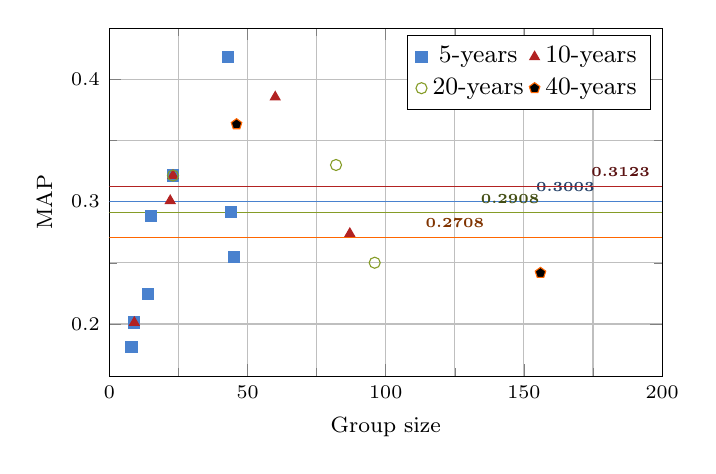
\begin{tikzpicture}
\begin{axis}[
        width= 8.6cm, %\textwidth,
        height=6cm, %5cm,
        xmin=0,xmax=200,
    %    ymin=0,ymax=1,
        grid = both,
        ylabel={MAP},
        xlabel={Group size},
        scatter/classes={
        	a={mark=square*,b},%
        	b={mark=triangle*,r},%
        	c={mark=o,draw=g},
        	d={mark=pentagon*,draw=o}
    	},
    	legend columns=2,
    	grid = both,
    	minor tick num=1,
    	tick label style={font=\fontsize{7}{9}\selectfont},
        label style = {font=\fontsize{8}{10}\selectfont},
        legend style={font=\fontsize{9}{11}\selectfont},
	]

	% \addplot[] is better than \addplot+[] here:
	% it avoids scalings of the cycle list
	\addplot[scatter,only marks,
		scatter src=explicit symbolic]
		coordinates {
			(9,0.2012)  [a]
			(44,0.2914) [a]
			(43,0.4181) [a]
			(45,0.2545)  [a]
			(15,0.2886)  [a]
			(14,0.2245)  [a]
			(8,0.1811)   [a]
			(23,0.3214) [a]
			(9,0.2012) [b]
			(87,0.2739) [b]
			(60,0.3855) [b]
			(22,0.3008) [b]
			(23,0.3214) [b]
			(96,0.2501) [c]
			(82,0.3300) [c]
			(23,0.3214) [c]
			(156,0.2418) [d]
			(46, 0.3633) [d]
		};
		\addplot[b,sharp plot,update limits=false] coordinates {(0,0.3003) (200,0.3003)} node[b!50!black, above] at (axis cs:165,0.3003) {\tiny{\textbf{0.3003}}}; 
		\addplot[r,sharp plot,update limits=false] coordinates {(0,0.3123) (200,0.3123)}node[r!50!black, above] at (axis cs:185,0.3123) {\tiny{\textbf{0.3123}}}; 
	    \addplot[g,sharp plot,update limits=false] coordinates {(0,0.2908) (200,0.2908)}node[g!50!black, above] at (axis cs:145,0.2908) {\tiny{\textbf{0.2908}}};  
		\addplot[o,sharp plot,update limits=false] coordinates {(0,0.2708) (200,0.2708)}node[o!50!black, above] at (axis cs:125,0.2708) {\tiny{\textbf{0.2708}}}; 
	
%	node[above] at (axis cs:0,0.26) {Houses};
		\legend{5-years,10-years,20-years,40-years}
\end{axis}
\end{tikzpicture}
% \vspace{-15pt}
\caption{Effect of groups granularity on the performance group profiling.\label{fig:Chart2}}
%  \vspace{-15pt}
 \end{figure}

\subsection{Effect of Rating Behaviour}
\label{sec:rb}
As we showed, using group-based information that is modeled by \acswlm helps to improve the performance of contextual suggestion. To study where does this improvement come from, we looked into the data to see in which cases adding group information helps and in which cases it is not effective. We observed that there is a correlation between the amount of improvement in contextual suggestion using group-based information and the rating behavior of users.

\begin{figure}[t]
\centering
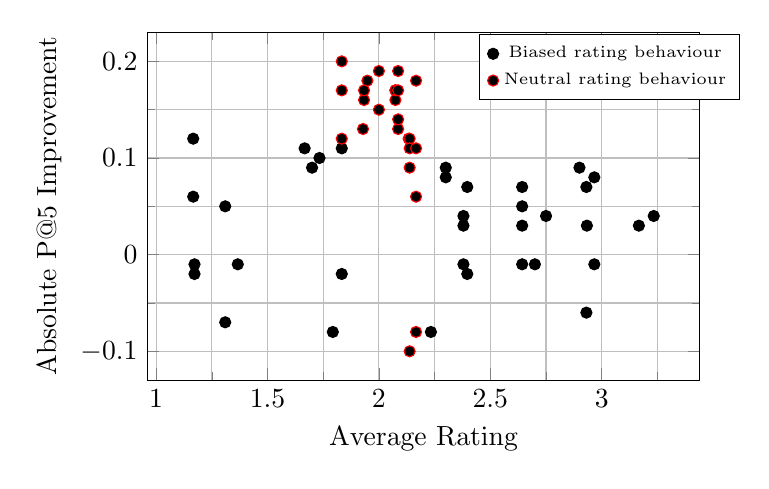
\begin{tikzpicture}
\begin{axis}[%
ylabel=Absolute P@5 Improvement ,
xlabel=Average Rating,
scatter/classes={%
    a={mark=*,draw=black},
    b={mark=*,draw=red}
    },
width= 8.6cm, %\textwidth,
height=6cm, %5cm,
grid = both,
legend columns=2,
grid = both,
minor tick num=1,
legend columns=1, 
legend style={
        at={(0.6,0.90)},
        anchor=west,
        font=\fontsize{6}{7}\selectfont,
        /tikz/column 2/.style={
            column sep=5pt,
        },
    },
% scatter/classes={
% 	a={mark=square*,draw=b},%
% 	b={mark=triangle*,draw=g},%
% },
]
\addplot[scatter,only marks,%
    scatter src=explicit symbolic]%
table[meta=label] {
x     y      label
1.1666666667	0.06	a
1.1666666667	0.12	a
1.1724137931	-0.01	a
1.1724137931	-0.02	a
1.3103448276	0.05	a
1.3103448276	-0.07	a
1.3666666667	-0.01	a
1.6666666667	0.11	a
1.7	0.09	a
1.7333333333	0.1	a
1.7931034483	-0.08	a
1.8333333333	0.11	a
1.8333333333	-0.02	a
1.8333333333	0.12	b
1.8333333333	0.17	b
1.8333333333	0.2	b
1.9285714286	0.13	b
1.9333333333	0.16	b
1.9333333333	0.17	b
1.9482758621	0.18	b
2	0.19	b
2	0.15	b
2.0740740741	0.17	b
2.0740740741	0.16	b
2.0740740741	0.17	b
2.0862068966	0.13	b
2.0862068966	0.19	b
2.0862068966	0.17	b
2.0862068966	0.14	b
2.1333333333	0.12	b
2.1379310345	0.12	b
2.1379310345	-0.1	b
2.1379310345	0.11	b
2.1379310345	0.09	b
2.1666666667	-0.08	b
2.1666666667	0.06	b
2.1666666667	0.11	b
2.1666666667	0.18	b
2.2333333333	-0.08	a
2.3	0.09	a
2.3	0.08	a
2.3793103448	0.03	a
2.3793103448	-0.01	a
2.3793103448	0.04	a
2.3965517241	0.07	a
2.3965517241	-0.02	a
2.6428571429	-0.01	a
2.6428571429	0.03	a
2.6428571429	0.05	a
2.6428571429	0.07	a
2.7	-0.01	a
2.75	0.04	a
2.9	0.09	a
2.9310344828	0.07	a
2.9310344828	-0.06	a
2.9333333333	0.03	a
2.9666666667	0.08	a
2.9666666667	-0.01	a
3.1666666667	0.03	a
3.2333333333	0.04	a
    };

\legend{Biased rating behaviour, Neutral rating behaviour}
\end{axis}
\end{tikzpicture}
\caption{\label{fig:gprates}Improvement of the performance of contextual suggestion by help of group profiles for users with different rating behavior.}
    \end{figure}

Figure~\ref{fig:gprates} shows the scatter plot of the change in $p@10$ after employing group-based information based on different rating tendency.
According to the plot, group-based information works better when the users have a neutral tendency in their rating (around rate 2) and it is less likely to help when users have rather strong biases by rating attraction with high or low rates. This could be due to the fact that in case of having neutral users, we have less strong information coming from their profile and then group-based information is compensating this lack of strong signals.
\section{Related Work}
In this section, we discuss related studies to the applications that we evaluated \acswlm on, i.e, in feedback in the retrieval task and group profiling in contextual suggestion. 

\subsection{Relevance Feedback}
It has been shown that there is a limitation on providing increasingly better results for retrieval systems only based on the original query~\citep{Rijsbergen:1986}. So, it is crucial to reformulate the search request using terms that reflect the user's information need to improve the performance of the retrieval systems. 
To address this issue, automatic feedback methods for information retrieval were introduced fifty years ago~\citep{Rocchio:1971} and have been extensively studied  during past decades.
%~\citep{Rijsbergen:1981,Robertson:1976,Salton:1985,Robertson:1991,Harman:1992,Buckley:1994,Lavrenko:2001,Zhai:SMM:2001,Ruthven:2003,Tao:2006, He:2009:ECIR,Lv:2009,He:2009:CIKM,Harman:2009,Carpineto:2012,Lv:2014}. 
As the earliest relevance feedback approach in information retrieval, the Rocchio method~\citep{Rocchio:1971} has been proposed in the vector processing environments for changing the query vector to be similar to the relevant documents vectors and dissimilar to the non-relevant documents vectors. 
Later, probabilistic methods have been proposed to select expansion terms from feedback documents based on a term weighting approach~\citep{Robertson:1976,Rijsbergen:1981}. With the development of language models, several feedback approaches have been proposed in this framework to improve the query language model~\citep{Zhai:SMM:2001,Tao:2006,Lavrenko:2001,Hiemstra:2004,Lv:2014}. 
The mixture model~\citep{Zhai:SMM:2001} is one of the well-known feedback methods in the language modeling framework, which empirically performs well. The idea is to extract a discriminative language model of feedback documents by decreasing weights of the background terms. 
As an extension to this model, the regularized mixture model has been proposed by \citet{Tao:2006}, which not only involves the query model in the estimated feedback model but also has document-specific mixing coefficients to let different documents have a different amount of background terms.

In the relevance model (RM)~\citep{Abdul-jaleel:2004,Lavrenko:2001} given the query, a model is estimated as a multinomial distribution over terms that indicates the likelihood of each term given the query as the evidence, based on the occurrences of the term together with the query terms in the feedback documents.  In a comparable study conducted by~\citet{Zhai:SMM:2001}, it has been shown that RM3 as a variant of the relevance model is one of the best performing methods which is strongly robust.
Divergence minimization~\citep{Zhai:SMM:2001} tries to estimate a feedback model that is close to the language model of every feedback document but far from the collection language model as an approximation of the non-relevant language model. This method generates a highly skewed feedback model, which makes it unable to perform well. \citet{Lv:2014} proposed the maximum-entropy divergence minimization model that, by adding an entropy term, regularizes the original divergence minimization model leading to significant improvements in the performance of the original method.

The parsimonious language model~\citep{Hiemstra:2004} is one of the models employed for feedback~\citep{Meij:2008,Hiemstra:2008:TREC,Kaptein:2008:TREC}. It tries to describe the feedback model using a smaller number of parameters. Similar to the mixture model, the common words in the collection are removed from the model in the estimation process, which leads to a more lean and mean language model.  \citet{Zamani:2016a}, considering the feedback problem as a recommendation problem, made use of matrix factorization in order for predicting expansion terms in a weighted manner.

Besides the ad hoc studies, there have been some initiatives aimed at studying the problem of (pseudo-)relevance feedback in detail. In 2003, Reliable Information Access (RIA) Workshop~\citep{Harman:2009,Warren:2004} 
%,Gu:2004:RIA,Montgomery:2004,Lynam:2004:RIA,Terra:2005
was organized with the goal of understanding the contributions of both system variability factors and topic variability factors to the overall retrieval variability in feedback. 
%Later on, in 2008, the Relevance Feedback track was intended as one the TREC tracks and it has been continued for two more years. The initial goal of the TREC Relevance Feedback track was evaluating and comparing different feedback methods~\citep{Buckley:2008:TREC}. In the next years, the tasks in TREC Relevance Feedback track focused on studying what is a good document for relevance feedback and how a system can recognize a good document~\citep{Buckley:2010:TREC}. 
In addition to the Relevance Feedback track, the Robust track in TREC defined one of the goals to improve the consistency of feedback systems by focusing on the poorly performing topics~\citep{Voorhees:2003:TREC}.

%Applying feedback deteriorates the performance of retrieval in some topics, especially in pseudo relevance feedback in which the performance of the feedback run strongly depends on the quality of the top documents in the initial run~\citep{Harman:2009,Collins-Thompson:2009}. 
%,Billerbeck:2003
%On the other hand, using some documents (even relevant documents) might harm the feedback performance~\citep{Terra:2005,Lv:2009:CIKM}.  
%Hence, there are some challenges in the feedback problem like how to determine whether applying the feedback improves the performance for a specific topic, and how to measure the quality of each feedback document and how to incorporate this information in the feedback process.
%
%\citet{He:2009:CIKM} proposed to examine to which degree the feedback documents is about the topic of the query using Entropy. In other work~\citep{He:2009:ECIR} they try to detect good feedback documents in PRF by grouping documents employing features like the probability of the query terms in the feedback document, the similarity of each feedback document with other feedback documents, and closeness of expansion terms to the original query terms. 
%\citet{Lee:2008} proposed to find the dominant documents from the initial run as better documents for PRF\@. 
%\citet{Tao:2004} proposed a two-stage mixture model in which taking the query as a relevant prior, feedback documents are divided into relevant and background documents and only the documents in the relevant group are employed for updating the query model. 
%\citet{Collins-Thompson:2007} tried to model feedback uncertainty to improve the robustness. They proposed to perform sampling over the feedback documents as well as the query to generate different sets of feedback documents and several query variants. Then, combining different feedback models from alternative sets, the robustness of the feedback model can be improved.

\medskip
Arguably, the key issue in feedback is robustness in terms of being able to deal with non-relevant terms from non-relevant or partially relevant documents. \acswlm addresses the robustness problem head on. This is achieved by using the information from the collection and other feedback documents to control the contribution of documents in the feedback model regarding their merit and to avoid the selection of non-relevant expansion terms.

\subsection{Group profiling for Content Customization}
Group profiling can help understand both explicit groups, like Facebook groups, and implicit groups, like groups extracted by community detection algorithms. There is a wide range of applications for group profiling, like understanding social structures~\citep{Tang:2011}, network visualization, recommender systems~\citep{Hu:2014,Shang:2014,Amer-Yahia}, and direct marketing~\citep{Custers:2003}. 

There is various research done on the task of group profiling which, given the individual attributes and preferences, aims to find out group-level shared preferences~\cite{Senot:2011,Masthoff:2011}.
\citet{Tang:2011} presented three methods for group profiling: \emph{Aggregation}, which tries to find features that are shared by the whole group; \emph{Differentiation}, which tries to extract features that can help to differentiate one group from others; and \emph{Egocentric differentiation}, which tries to extract features that can help to differentiate members of one group from the neighbour members. In recent work, \citet{Hu:2014} proposed a deep-architecture model to learn a high level representation of group preferences.

For group recommendation,  there is research on building a model of a group by forming a linear combination of the individual models~\citep{Jameson:2007}. Some of them construct the group's preference model on the basis of individual preference models, using a notion of distance between preference models~\citep{Yu:2006}. Some approaches try to divide the group into several categories of homogeneous users and specify the preference model for each subgroup. Then they create the group model as a weighted average of the subgroup models, with the weights reflecting the importance of the subgroups~\citep{Ardissono:2003}.


\section{Conclusion} 
In this chapter, inspired by the discussion on the early work by~\citet{Luhn:1958} about \emph{significant words}, we proposed \emph{\swlms}\ (\acswlm) to estimate a representation for a set of documents that captures significant terms by avoiding the distracting effect of common observation as well as rare observation.

We showed that utilizing \acswlm as the feedback model presents promising performance on both true and pseudo relevance feedback. Analysing the results, we indicated that the strength of \acswlm in feedback is due the fact that it is capable of controlling the contribution of feedback documents in the feedback model based on their level of relevancy which copes with the problem of topic drift in query expansion. We assessed the robustness of \acswlm in different experiments and showed that in PRF, both it has the least vulnerability against noise in the data in the form of non-relevant terms and/or non-relevant documents in feedback set.
%
We also employed \acswlm as a group profiling approach for the task of contextual suggestion, and our experimental results showed using the group representations estimated by \acswlm, we can improve the performance of content customization. 

We named our model, significant ``words'' language model in honor of \citeauthor{Luhn:1958}, however, it could be employed in non-textual environments, since in general the idea is to extract significant ``features'' representing the shared essence of a group of entities.

% connecting chapter 2 to chapter 3:
The process of estimating \acswlm leads to a sparse model, i.e. $\theta_{sw}$ assigns zero probability to many terms that are identified as either too general or too specific for representing and entity. Sparsity has a central role in human episodic memory.  In human brain, sparse activities is important to separate representations as it reduces the risk that a single neuron holds representations of two overlapping memories\citep{cho2018blockchain}. In addition to human brain, for many systems, sparsity is a desirable property, like for instance sparse representations are easier to interpret or sparse representations are more likely to posses separability which is important for collision resistance hash functions. 
In Chapter~\ref{chap:3}, we extend \acswlm to hierarchically structured entities and discuss separability as a key objective for learning the representations.


